\documentclass[notitlepage]{article}
\usepackage{amsmath, amssymb}
\usepackage{enumerate}
\usepackage[margin=1in]{geometry}
\usepackage{tikz}
\usepackage{standalone}
\usepackage{graphicx}
\usepackage{subfig}
\usepackage{cases}
\usepackage{xcolor}
\usepackage{multirow}
\usepackage{cancel}
\usepackage{pgfplots}

\usetikzlibrary{shapes.geometric, decorations.markings, arrows.meta}
\definecolor{gamegreen}{RGB}{58, 107, 34}
\definecolor{trafficgreen}{RGB}{34, 139, 34}
\definecolor{trafficyellow}{RGB}{204, 170, 0}
\definecolor{gameblue}{RGB}{0, 102, 204}
\definecolor{gamered}{RGB}{204, 51, 34}

\pgfplotsset{compat=1.18} 

\newcommand{\bluestrike}[1]{{\color{blue}\xcancel{\color{black}#1}}}
\newcommand{\redstrike}[1]{{\color{red}\xcancel{\color{black}#1}}}

\setlength\parindent{0pt}

\begin{document}
Author: Jacky Leung

This is a set of notes for ECON 4124: Applied Game Theory at HKUST. Content is based on Professor Wu Qinggong's lecture notes and course materials, with a few additional examples by the author.

%These notes are for ECON 4124: Applied Game Theory at HKUST. The content is based on Professor Wu Qinggong’s lecture notes and course materials, with a few additional examples added by the author (marked with \#). While some examples in the lecture notes adapt classic games to modern settings, the original game names are retained here to make online searching easier, while still largely following the lecture notes' framing.

\section{Introduction}

\begin{itemize}
    \item What is a game?
    \begin{itemize}
        \item One or more \textbf{players} take \textbf{actions}, which lead to some \textbf{outcomes}.
    \end{itemize}
    \item How can we classify different types of games?
    \begin{itemize}
        \item Number of players: Single-player or N-player.
        \item Move sequences: Static (everyone moves together) or Dynamic (everyone takes turn to move).
        \item Information: Perfect/Complete or Imperfect/Incomplete.
        \item Number of rounds: One-shot or Repeated.
        \item Other classifications: Zero-sum or Non-zero-sum, Deterministic or Probabilistic...
    \end{itemize}
    \item In this course, we primarily focus on N-player games with different move sequences and information.
    \item Loosely speaking, we will be following the framework recognized by the 1994 Nobel Prize in Economics: John Nash provided the foundation for equilibrium in static games, Reinhard Selten extended this to dynamic, multi-stage games, and John Harsanyi incorporated games with incomplete information.
\end{itemize}

\subsection{Preferences and Utility}

\begin{itemize}
    \item How do players make choices in a game?
    \begin{itemize}
        \item If a player finds choice \(a\) better than choice \(b\), then naturally they would choose \(a\) over \(b\).
    \end{itemize}
    \item We use the following notations to represent one's pairwise preferences:
    \begin{itemize}
        \item \(a \succ b\): \(a\) is strictly better than \(b\).
        \item \(a \succeq b\): \(a\) is weakly better than (at least as good as) \(b\).
        \item \(a \sim b\): \(a\) is as good as \(b\).
    \end{itemize}
    \item Consider an example of a simple one-player game.
    \item \textbf{Example 1.1. Super Mario.} You are playing the classic video game \textit{Super Mario}. On the edge of the cliff, you have two choices: to jump or to keep walking.
    \begin{itemize}
        \item As we will do so over the course, we need to mathematically formalize the game.
        \item The choices of actions are defined as a choice set: \[A = \{jump, walk\}\]
        \item The outcome that will happen is also a set: \[X = \{survive, die\}\]
        \item To connect the two, a simple function \(A \to X\) is needed, where \[jump \to survive \text{ and } walk \to die\]
        \item Before making the decision, you might have no view about the actions per se, but you have preferences about the outcome: \[survive \succ die\]
        \item Then, you have your derived preference about the actions: \[jump \succ walk\]
        \item Therefore, a rational you should choose to jump over walking.
        \item Because an action must leads to an outcome, to simplify our mathematical derivation, we simply talk about preferences over the actions \(A\) most of the time. 
    \end{itemize}
    \item For simple situations, we can just represent the preferences by ranking. For example, \(win \succ tie \succ lose\).
    \begin{itemize}
        \item \textit{Remark.} We always assume preferences to be transitive. That is, if \(a \succ b\) and \(b \succ c\), then \(a \succ c\).
    \end{itemize}
    \item Things might get complicated when we have more, or even infinite choices. (Think about choosing a real number!)
    \item Economists use something called a utility (or payoff) function that assigns each action \(a \in A\) a number: \[u: A \to \mathbb{R}\]
    \item \(u\) represents all preferences over \(A\). The higher utility, the better the action: \[\forall a, b \in A: a \succeq b \iff u(a) \ge u(b)\]
    \item To choose the best action out of all, we find the one that maximizes the utility by solving: \[\max_{a\in A}u(a)\]
    \item Utility function is not unique; there can be multiple utility functions representing the same preferences, as long as the relative ordering are the same.
    \begin{itemize}
        \item For example, $u(win) = 1, u(lose) = 0$ and $v(win) = 100, v(lose) = -100$ are the same.
    \end{itemize}
    \item In game theory, sometimes seemingly trivial facts are not actually trivial and need to be proved.
    \item \textbf{Theorem 1.1.} If \(u: A \to \mathbb{R}\) and \(v: A \to \mathbb{R}\) are two utility functions representing the same preferences over \(A\), then:
    \[
    \max_{a\in A}u(a)
    \]
    and
    \[
    \max_{a\in A}v(a)
    \]
    have the same solution.
    \begin{itemize}
        \item \textit{Proof.} Since \(u\) and \(v\) represent the same preferences over \(A\), for all \(a, b \in A\), \(a \succeq b\) if and only if \(u(a) \ge u(b)\) and \(v(a) \ge v(b)\). Suppose \(a^*\) is a solution to \(\max_{a\in A}u(a)\), then \(a^* \succeq a\) for every \(a \in A\). This implies that \(v(a^*) \ge v(a)\) for every \(a \in A\), and thus \(a^*\) is a solution to \(\max_{a\in A}v(a)\).
    \end{itemize}
\end{itemize}

\section{Static Games and the Nash Equilibrium}

\begin{itemize}
    \item We start with an example of a two-player game.
    \item \textbf{Example 2.1. Penalty Shootout (Matching Pennies).} Kicker Messi is facing off goalkeeper De Gea in a Penalty Shootout. Each of them choose a direction (left or right) to kick or to dive.
    \begin{itemize}
        \item Messi's actions: \(\{\leftarrow_M, \rightarrow_M\}\)
        \item De Gea's actions: \(\{\leftarrow_D, \rightarrow_D\}\)
        \item Like the last example, the players have preferences on the outcome: \(\{Goal, No \;goal\}\), where \(Goal \succ_M No \;goal\) for Messi and \(No \;Goal \succ_D Goal\) for De Gea.
        \item However, each of them cannot directly derive the outcome from their own action directly, but rather by both of their actions:
        \[
        Goal 
        \begin{cases}
            (\leftarrow_M, \rightarrow_D) \\
            (\rightarrow_M, \leftarrow_D)
        \end{cases}
        \]
        \[
        No\;Goal 
        \begin{cases}
            (\leftarrow_M, \leftarrow_D) \\
            (\rightarrow_M, \rightarrow_D)
        \end{cases}
        \]
        \item Each vector of their actions, \((a_M, a_D)\), is called an \textbf{action profile}.
        \item The set of all possible action profiles is the Cartesian product of all players' action sets: \(A_M \times A_D\).
        \item Since each action profile leads to one outcome, the players have preferences over action profiles. For example, for Messi, \((\leftarrow_M, \rightarrow_D) \sim (\rightarrow_M, \leftarrow_D) \succ (\leftarrow_M, \leftarrow_D) \sim (\rightarrow_M, \rightarrow_D)\).
        \item Their preferences can be represented by utility functions:

        For Messi:
        \[
        \begin{cases}
            (Goal) \; u_M(\leftarrow_M, \rightarrow_D) = u_M(\rightarrow_M, \leftarrow_D) = 1 \\
            (No \; Goal ) \; u_M(\leftarrow_M, \leftarrow_D) = u_M(\rightarrow_M, \rightarrow_D) = -1
        \end{cases}
        \]
        For De Gea:
        \[
        \begin{cases}
            (No\;Goal) \; u_D(\leftarrow_M, \leftarrow_D) = u_D(\rightarrow_M, \rightarrow_D) = 1 \\
            (Goal ) \; u_D(\leftarrow_M, \rightarrow_D) = u_D(\rightarrow_M, \leftarrow_D) = -1
        \end{cases}
        \]
        \item The utility values can be summarized using a \textbf{payoff matrix}, also known as a \textbf{normal-form game}:

        \begin{table}[h]
        \begin{center}
        \begin{tabular}{llcc}
        &&
        \multicolumn{2}{c}{\textcolor{blue}{De Gea}}  \\&& 
        \textcolor{blue}{$\leftarrow_D$} & 
        \textcolor{blue}{$\rightarrow_D$} 
        \\ \cline{3-4} 
        \multirow{2}{*}{\textcolor{red}{Messi}} & 
        \multicolumn{1}{c|}{\textcolor{red}{$\leftarrow_M$}} & 
        \multicolumn{1}{c|}{(\textcolor{red}{-1}, \textcolor{blue}{1})} &
        \multicolumn{1}{c|}{(\textcolor{red}{1}, \textcolor{blue}{-1})} 
        \\ \cline{3-4} & 
        \multicolumn{1}{c|}{\textcolor{red}{$\rightarrow_M$}} & 
        \multicolumn{1}{c|}{(\textcolor{red}{1}, \textcolor{blue}{-1})} &
        \multicolumn{1}{c|}{(\textcolor{red}{-1}, \textcolor{blue}{1})} 
        \\ \cline{3-4} 
        \end{tabular}
        \end{center}
        \end{table}
    \end{itemize}
\end{itemize}

\begin{itemize}
    \item Now, we can formalize what elements constitute a game in general.
    \begin{itemize}
        \item A set of players: \(I\).
        \item Each player \(i \in I\) has a set of available actions: \(A_i\).
        \item An action profile \(\mathbf{a}\) is a vector of actions taken by each player: \((a_i)_{i \in I} = (a_1, \dots, a_n)\), or from the point of view of player \(i\), \((a_i, \mathbf{a}_{-i})\).
        \item The set of all possible action profiles: \(\mathbf{A} = \times_{i \in I}A_i\).
        \item Each player has their own preferences \(\succeq_i\) over \(\mathbf{A}\), which can be represented by utility function \(u_i\).
        \item Again, preferences over action profiles alone is sufficient to represent the outcomes.
    \end{itemize}
    \item We continue with what is perhaps the most well-known example in game theory.
    \item \textbf{Example 2.2. Prisoner's Dilemma.} Two criminals, Bane and Joker, are arrested and locked in separate interrogation rooms. They must decide whether to defect and betray each other to receive a shorter jail sentence, or to remain silent and cooperate.
    \begin{itemize}
        \item Players: \{Bane, Joker\}
        \item Actions: \(A_B = A_J = \{Cooperate, Defect\}\)
        \item Outcomes:
        \[
        \begin{cases}
            \text{Both cooperate: 1 year sentence each} \\
            \text{One defect, one cooperate: The traitor is freed, the other serves 3 years} \\
            \text{Both defect: 2 years sentence each}
        \end{cases}
        \]
        \item The criminals prefer shorter sentence:
        \[
        0\text{ years}\succ 1\text{ year} \succ 2\text{ years} \succ 3\text{ years}
        \]
        \item So we can derive the preferences over the action profiles. Furthermore, we can assign the negative of the number of years for the utility. For example, for \textcolor{red}{Bane}:
        \[
        \underbrace{(\textcolor{red}{D}, \textcolor{blue}{C})}_{0} \succ \underbrace{(\textcolor{red}{C}, \textcolor{blue}{C})}_{-1} \succ \underbrace{(\textcolor{red}{D}, \textcolor{blue}{D})}_{-2} \succ \underbrace{(\textcolor{red}{C}, \textcolor{blue}{D})}_{-3}
        \]
        \item The payoff matrix is therefore:

\begin{table}[h]
\begin{center}
\begin{tabular}{llcc}
&&
\multicolumn{2}{c}{\textcolor{blue}{Joker}}  \\&& 
\textcolor{blue}{Cooperate} & 
\textcolor{blue}{Defect} 
\\ \cline{3-4} 
\multirow{2}{*}{\textcolor{red}{Bane}} & 
\multicolumn{1}{c|}{\textcolor{red}{Cooperate}} & 
\multicolumn{1}{c|}{(\textcolor{red}{-1}, \textcolor{blue}{-1})} &
\multicolumn{1}{c|}{(\textcolor{red}{-3}, \textcolor{blue}{0})} 
\\ \cline{3-4} & 
\multicolumn{1}{c|}{\textcolor{red}{Defect}} & 
\multicolumn{1}{c|}{(\textcolor{red}{0}, \textcolor{blue}{-3})} &
\multicolumn{1}{c|}{(\textcolor{red}{-2}, \textcolor{blue}{-2})} 
\\ \cline{3-4} 
\end{tabular}
\end{center}
\end{table}

    \end{itemize}
    \item To familiarize yourself with the payoff matrix, you should be able to explain this game alone by just looking at it:
    \item \textbf{Example 2.3. Battle of Sexes.} Adam and Eve are deciding which movie to watch.

\begin{table}[h]
\begin{center}
\begin{tabular}{llcc}
&&
\multicolumn{2}{c}{\textcolor{blue}{Eve}}  \\&& 
\textcolor{blue}{Horror} & 
\textcolor{blue}{Romance} 
\\ \cline{3-4} 
\multirow{2}{*}{\textcolor{red}{Adam}} & 
\multicolumn{1}{c|}{\textcolor{red}{Horror}} & 
\multicolumn{1}{c|}{(\textcolor{red}{2}, \textcolor{blue}{1})} &
\multicolumn{1}{c|}{(\textcolor{red}{0}, \textcolor{blue}{0})} 
\\ \cline{3-4} & 
\multicolumn{1}{c|}{\textcolor{red}{Romance}} & 
\multicolumn{1}{c|}{(\textcolor{red}{0}, \textcolor{blue}{0})} &
\multicolumn{1}{c|}{(\textcolor{red}{1}, \textcolor{blue}{2})} 
\\ \cline{3-4} 
\end{tabular}
\end{center}
\end{table}
\end{itemize}

\subsection{Nash Equilibrium}

\begin{itemize}
    \item One key question we should ask is: What will happen in the game, or formally, which action profiles will realize?
    \begin{itemize}
        \item In fact, it is easier to tell what will not happen instead.
        \item For example, will the action profile (\textcolor{red}{Horror}, \textcolor{blue}{Romance}) realize in the \textit{Battle of Sexes}?
        \item No: If Adam knows Eve will choose Romance, he must choose Romance over Horror for a higher utility.
        \[
        u_A(\textcolor{red}{Romance}, \textcolor{blue}{Romance}) = 1 > 0 = u_A(\textcolor{red}{Horror}, \textcolor{blue}{Romance})
        \]
        \item That means under this action profile, at least one player can change their action to get higher utility. Formally, this is called a \textbf{profitable (unilateral) deviation}.
    \end{itemize}
    \item If we rule out all action profiles with profitable deviations, then we are left with what can be realized.
    \item Such action profile is a (pure strategy) \textbf{Nash equilibrium}.
    \item \textbf{Definition 2.1.} A (pure strategy) action profile \(\mathbf{a^*} \in \mathbf{A}\) is a Nash equilibrium if and only if for every player \(i\) and every action \(a_i \in A_i\):
    \[
    u_i(a^*_i,\mathbf{a}^*_{-i}) \ge u_i(a_i,\mathbf{a}^*_{-i})
    \]
    \item How to find a Nash equilibrium in practice?
    \begin{enumerate}
        \item For each player \(i\), for every possible actions \(\mathbf{a}_{-i}\) the opponent(s) can make, we rule out all actions that allow profitable deviations; in other words, we only keep the actions that give the highest utility. These are called \textbf{best responses}.
        \item The action profile(s) we are left with must be the Nash equilibria, since none of the players can deviate in those action profiles.
    \end{enumerate}
    \item For simple games with limited actions, we can just put ticks for the best responses.
    \item For example, in the \textit{Prisoner's Dilemma}, we think about \textcolor{red}{Bane}:
    \begin{itemize}
        \item If \textcolor{blue}{Joker} chooses to cooperate, \textcolor{red}{Bane}'s best response is to \textcolor{red}{defect} over \textcolor{red}{cooperate}:
        \[
        u_B(\textcolor{red}{D}, \textcolor{blue}{C}) = 0 > -1 = u_B(\textcolor{red}{C}, \textcolor{blue}{C})
        \]
        \item If \textcolor{blue}{Joker} chooses to defect, \textcolor{red}{Bane}'s best response is still to \textcolor{red}{defect} over \textcolor{red}{cooperate}:
        \[
        u_B(\textcolor{red}{D}, \textcolor{blue}{D}) = -2 > -3 = u_B(\textcolor{red}{C}, \textcolor{blue}{C})
        \]
        \item So, Bane's best response is to always defect no matter what Joker does. Since the game works in the exact same way for Joker, we know that always defecting is also the optimal strategy for him.
        \item Therefore, we are left with the only Nash equilibrium: \((\textcolor{red}{D}, \textcolor{blue}{D})\), which has two ticks in our payoff matrix.
    \end{itemize}
\end{itemize}

\begin{table}[h]
\begin{center}
\begin{tabular}{llcc}
&&
\multicolumn{2}{c}{\textcolor{blue}{Joker}}  \\&& 
\textcolor{blue}{Cooperate} & 
\textcolor{blue}{Defect} 
\\ \cline{3-4} 
\multirow{2}{*}{\textcolor{red}{Bane}} & 
\multicolumn{1}{c|}{\textcolor{red}{Cooperate}} & 
\multicolumn{1}{c|}{(\textcolor{red}{-1}, \textcolor{blue}{-1})} &
\multicolumn{1}{c|}{$(\textcolor{red}{-3}, \textcolor{blue}{0^\checkmark})$}
\\ \cline{3-4} & 
\multicolumn{1}{c|}{\textcolor{red}{Defect}} & 
\multicolumn{1}{c|}{$(\textcolor{red}{0^\checkmark}, \textcolor{blue}{-3})$}  &
\multicolumn{1}{c|}{$(\textcolor{red}{-2^\checkmark}, \textcolor{blue}{-2^\checkmark})$}
\\ \cline{3-4} 
\end{tabular}
\end{center}
\end{table}

\begin{itemize}
    \item Interestingly, the seemingly more promising option \((\textcolor{red}{C}, \textcolor{blue}{C})\) which gives higher utility to both will not happen at all, because both of them know that defecting must make them better off.
    \item Another counterintuitive example:
    \item \textbf{Example 2.4. Voting Game.} Three voters are choosing between candidates A and B using majority rule. Even if all voters prefer candidate A over candidate B, the action profile where all three vote for B is still a Nash equilibrium: no individual voter can change the outcome by unilaterally changing their own vote alone, so a deviation is unprofitable for all them.
    \begin{itemize}
        \item The paradox of voting: If you know for certain that your one vote wouldn't change the outcome, why do you still vote?
    \end{itemize}
\end{itemize}

\subsection{Best Response}

\begin{itemize}
    \item For each player \(i\), we can formalize best response as a \textbf{best response function} \(B_i : \mathbf{A}_{-i} \to 2^{A_i}\),
    \[
    B_i(\mathbf{a}_{-i}) = \{a_i \in A_i: u_i(a_i,\mathbf{a}_{-i}) \ge u_i(a'_i,\mathbf{a}_{-i}) \;\forall a'_i \in A_i\}
    \]
    \item The output of \(B_i\) is a set: For some \(\mathbf{a}_{-i}\), \(B_i(\mathbf{a}_{-i})\) can have multiple, or sometimes even zero best responses.
    \begin{itemize}
        \item \textit{Remark.} But for convenience, we sometimes write something like \(B_i = 1\) instead of \(\{1\}\) if the best response is unique.
    \end{itemize}
    \item Now, we can prove something we discussed verbally earlier from definition.
    \item \textbf{Theorem 2.1.} An action profile \(\mathbf{a}^*\) is a Nash equilibrium if and only if for every player \(i\),
    \[
    a^*_i \in B_i(\mathbf{a}^*_{-i})
    \]
    \begin{itemize}
        \item \textit{Proof.} If: Suppose \(a^*_i \in B_i(\mathbf{a}^*_{-i})\) for every player \(i\), then \(u_i(a_i^*,\mathbf{a}_{-i}^*) \ge u_i(a_i,\mathbf{a}_{-i}^*)\) for all \(a_i \in A_i\), so by definition \(\mathbf{a}^*\) is a Nash equilibrium.

        Only if: Suppose \(\mathbf{a}^*\) is a Nash equilibrium, then \(u_i(a_i^*,\mathbf{a}_{-i}^*) \ge u_i(a_i,\mathbf{a}_{-i}^*)\) for all \(a_i \in A_i\), so by definition \(a^*_i \in B_i(\mathbf{a}^*_{-i})\) for every player \(i\).
    \end{itemize}
    \item For a two-player game, an action profile \((a_1^*, a_2^*)\) is a Nash equilibrium if and only if:
    \[
    \begin{cases}
        a_1^* \in B_1(a_2^*) \\
        a_2^* \in B_2(a_1^*)
    \end{cases}
    \]
    \item The tick method is one special application of this intersection method, as all actions we tick are best responses.
    \item With this being formalized, we can deal with some more complicated games, like games with continuous, and therefore infinite choices.
    \item \textbf{Example 2.5. Cournot Duopoly.} Two homogeneous firms producing the same goods are deciding the amount of goods to produce: \(q_i \in \mathbb{R}^+\). The goods have the following standard downward-sloping market demand function:
    \[
    P(Q) = \max(a-Q,0)
    \]
    where \(a\) is a positive constant and \(Q = q_1 + q_2\).

    Assume both firms have the same constant marginal cost \(c\). We can simply treat maximizing profit as maximizing utility, where:
    \begin{align*}
    u_i(q_i, q_{-i}) &= P \cdot q_i - c \cdot q_i \\
    &=
    \begin{cases}
         (a - q_i - q_{-i} - c)q_i &\text{if } q_i + q_{-i} \le a \\
         0 &\text{if } q_i + q_{-i} > a
    \end{cases}
    \end{align*}
    We solve the maximization problem for Firm 1 by first order condition. If \(q_1 + q_2 \le a\):
    \begin{align*}
        \frac{\partial u_1}{\partial q_1}\left((a - q_1 - q_2 - c)q_1\right) &= 0 \\
        a - 2q_1 - q_2 - c &= 0 \\
        q_1^* &= \frac{1}{2}(a - q_2 - c)
    \end{align*}
    Given that Firm 1 maximizes utility at \(\max\left(\frac{1}{2}(a - q_2 - c),0\right)\), their best response is exactly \(B_1(q_2) = \max\left(\frac{1}{2}(a - q_2 - c),0\right)\). Similarly, \(B_2(q_1) = \max\left(\frac{1}{2}(a - q_1 - c),0\right)\).

    By the intersection method, we solve for the system:
    \[
    \begin{cases}
    q_1 = \max\left(\frac{1}{2}(a - q_2 - c),0\right) \\
    q_2 = \max\left(\frac{1}{2}(a - q_1 - c),0\right)
    \end{cases}
    \]
    Solving, or graphically, we have the Nash equilibria:
    \[
    q_1^* = q_2^* = 
    \begin{cases}
    \frac{1}{3}\left(a-c\right) &\text{if } a \ge c \\
    0  &\text{if } a < c
    \end{cases}
    \]

    \newpage
    \begin{figure}[h]
    \centering
    \resizebox{0.5\textwidth}{!}{
    \documentclass{standalone}
\usepackage{tikz}

\begin{document}
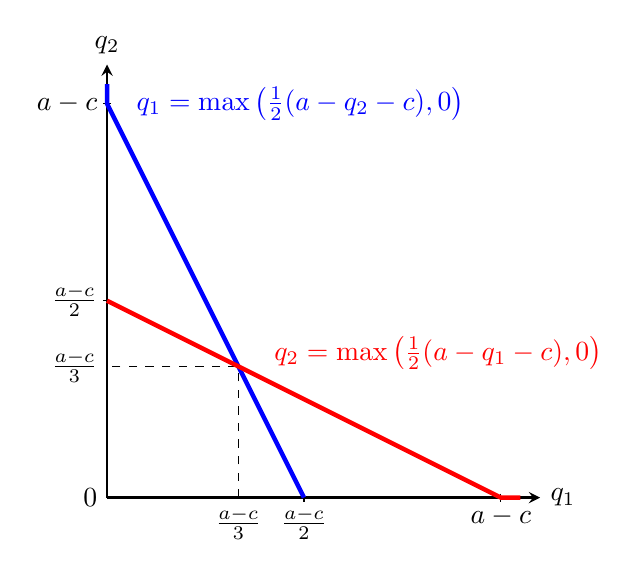
\begin{tikzpicture}[scale=5, >=stealth]

    % Axes
    \draw[->, thick] (0,0) -- (1.1,0) node[right] {$q_1$};
    \draw[->, thick] (0,0) -- (0,1.1) node[above] {$q_2$};

    % Axis Labels / Ticks
    \node[left] at (0,0) {$0$};
    \node[below] at (0.5,0) {$\frac{a-c}{2}$};
    \node[below] at (1,0) {$a-c$};
    \node[left] at (0,0.5) {$\frac{a-c}{2}$};
    \node[left] at (0,1) {$a-c$};

    % Tick marks
    \draw (0.5,0.01) -- (0.5,-0.01);
    \draw (1,0.01) -- (1,-0.01);
    \draw (0.01,0.5) -- (-0.01,0.5);
    \draw (0.01,1) -- (-0.01,1);

    % Dashed projection lines for Nash Equilibrium
    \draw[dashed] (1/3, 0) node[below] {$\frac{a-c}{3}$} -- (1/3, 1/3) -- (0, 1/3) node[left] {$\frac{a-c}{3}$};

    % Reaction Function 1 (Blue): q1 = max( (a - c - q2)/2 , 0 )
    % Vertical along q2-axis for q2 >= a-c, then down to q1 = (a-c)/2 at q2 = 0
    \draw[blue, ultra thick] (0, 1.05) -- (0, 1) -- (0.5, 0);

    % Reaction Function 2 (Red): q2 = max( (a - c - q1)/2 , 0 )
    % From q2 = (a-c)/2 at q1 = 0 down to q1 = a-c, then horizontal along q1-axis for q1 >= a-c
    \draw[red, ultra thick] (0, 0.5) -- (1, 0) -- (1.05, 0);

    % Legend / Function Labels
    \node[blue, right] at (0.05, 1) {$q_1 = \max \left( \frac{1}{2}(a - q_2 - c), 0 \right)$};
    \node[red, above right] at (0.4, 0.3) {$q_2 = \max \left( \frac{1}{2}(a - q_1 - c), 0 \right)$};

\end{tikzpicture}
\end{document}

    }
    \end{figure}

    \item \textbf{Example 2.6. Hotelling Model.} On a 1-km beach, represented by the interval $[0, 1]$ on the number line, two hot dog sellers are deciding where to place their carts: \(a_i \in [0,1]\). Customers are uniformly distributed along this interval, and each customer goes to whichever cart is closer to them. In other words, each seller aims to capture as much territory as possible, securing all customers closest to their cart while losing the remaining customers to their competitor.
    
    \begin{figure}[h]
    \centering
    \resizebox{0.5\textwidth}{!}{
    \documentclass[tikz, border=10pt]{standalone}
\usepackage{tikz}

\begin{document}
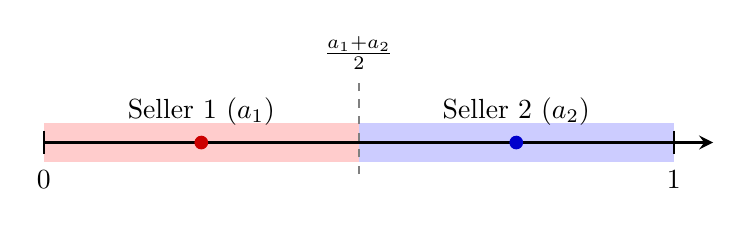
\begin{tikzpicture}[>=stealth]
  % Define coordinates (scaled manually to avoid distorting shapes)
  \def\xmin{0}
  \def\xmax{8}
  \def\sone{2}      % s_1 at 0.25
  \def\stwo{6}      % s_2 at 0.75
  \def\midpoint{4}  % Midpoint at 0.5

  % Color Regions (Occupied territory)
  \fill[red!20] (\xmin,-0.25) rectangle (\midpoint,0.25);
  \fill[blue!20] (\midpoint,-0.25) rectangle (\xmax,0.25);

  % Midpoint divider line
  \draw[dashed, thick, gray] (\midpoint,-0.4) -- (\midpoint,0.8);
  \node[above, black] at (\midpoint, 0.8) {$\frac{a_1 + a_2}{2}$};

  % Main Number Line
  \draw[very thick, ->] (\xmin,0) -- (\xmax + 0.5,0);

  % Endpoints
  \draw[thick] (\xmin, 0.15) -- (\xmin, -0.15) node[below=2pt] {$0$};
  \draw[thick] (\xmax, 0.15) -- (\xmax, -0.15) node[below=2pt] {$1$};

  % Store Locations (s1 and s2 as true circles)
  \node[circle, fill=red!80!black, inner sep=1.75pt, label={above:Seller 1 ($a_1$)}] at (\sone,0) {};
  \node[circle, fill=blue!80!black, inner sep=1.75pt, label={above:Seller 2 ($a_2$)}] at (\stwo,0) {};

  % Region Labels
  %\node[red!80!black, font=\bfseries] at (\midpoint/2, -0.6) {Seller 1 Market Share};
  %\node[blue!80!black, font=\bfseries] at (\midpoint + \midpoint/2, -0.6) {Seller 2 Market Share};

\end{tikzpicture}
\end{document}
    }
    \end{figure}

    Their utility is simply the length of the interval they occupy:
    \[
    u(a_i, a_{-i}) = 
    \begin{cases}
        \frac{a_i + a_{-i}}{2} &\text{if } a_i < a_{-i} \\
        \frac{1}{2} &\text{if } a_i = a_{-i} \\
        1 - \frac{a_i + a_{-i}}{2} &\text{if } a_i > a_{-i}
    \end{cases}
    \]
    There are two similar ways to find the Nash equilibrium.

    \begin{enumerate}
        \item Exhaustion: We look at all possible action profiles.
        \begin{itemize}
            \item \(a_i \ne a_{-i}\): Not NE; a seller can deviate towards the competitor to expand their territory.
            \item \(a_i = a_{-i} \ne 0.5\): Not NE; a seller can deviate towards the center to expand their territory.
            \item \(a_i = a_{-i} = 0.5\): The only NE.
        \end{itemize}
        \item Best response: Best response can be an empty set (\(\emptyset\)). For example, \(B_1(0.3)\) is empty.
        \begin{itemize}
            \item Any \(a_1 \le 0.3\) is not as good as \(a_1 = 0.4 \implies\) Profitable deviation.
            \item Any \(a_1 > 0.3\) is not as good as \(\frac{a_1+0.3}{2} \implies\) Profitable deviation.
        \end{itemize}
        We can verify that \(B_1(0.5) = 0.5\) is the only place where best response is nonempty. By intersection, (0.5, 0.5) is a NE.
    \end{enumerate}
\end{itemize}

\subsection{Randomization and Mixed Strategy}

\begin{itemize}
    \item Let's go back to discuss utility.
    \item So far we have been choosing from deterministic items (we get what we choose), what if we include lotteries?
    \item Consider a set of holiday destinations, Vienna, Paris, or stay at Home, where you have \(u(V) = 3, u(P) = 2, u(H) = 1\).
    \item We add a lottery to your choices: 10\% Vienna or 90\% Home \(= 0.1V + 0.9H\).
    \item Intuitively, we should know \(V \succ 0.1V + 0.9H \succ H\). But \(0.1V + 0.9H \succ \text{or} \prec P\)?
    \item To get to the preferences, we first formalize what a lottery is.
    \item A lottery can be defined as a probability function:
    \[
    \sigma: A \to [0,1] \text{ s.t. } \sum_{a \in A}\sigma(a) = 1
    \]
    \item For example, \(\sigma(V) = 0.1, \sigma(P) = 0, \sigma(H) = 0.1\).
    \begin{itemize}
        \item \textit{Remark.} Deterministic outcomes can also be expressed as lotteries; for example, \(\sigma(V) = 1, \sigma(P) = 0, \sigma(H) = 0\). This is called \textbf{degenerate}.
    \end{itemize}
    \item To generalize preferences over lotteries, we don't just focus on one or two lotteries, but all possible ones:
    \[
    \Delta(A) = \left\{\sigma:A \to [0,1] \text{ s.t. } \sum_{a \in A}\sigma(a) = 1\right\}
    \]
    For example,
    \[
    \Delta(\{V, P, H\}) = \left\{\underbrace{x}_{\sigma(V)},\overbrace{y}^{\sigma(P)},\underbrace{z}_{\sigma(H)} \text{ s.t. } x,y,z \in [0,1], x+y+z=1 \right\}
    \]
    \item Then, we can use \textbf{expected utility} to represent our preferences over lotteries, \(U: \Delta(A) \to \mathbb{R}\),
    \[
    U(\sigma) = \sum_{a \in A}\sigma(a)u(a)
    \]
    \begin{itemize}
        \item \textit{Remark.} Some literature defines expected utility using random variables with the expression \(\mathbb{E}[u(X)]\). While that formal definition is more mathematically complex, the two approaches are connected simply by letting \(\sigma(a) = \mathbb{P}(X = a)\).
    \end{itemize}
    \item \(U\) is also called the von Neumann-Morgenstern (vNM) utility function, which links up with the Bernoulli utility function \(u\).
    \item Then we can calculate the expected utility in the previous example:
    \[
    U(P) = 2 > 0.1\cdot3 + 0.9\cdot1 = 1.2 = U(0.1V+0.9H)
    \]
    which implies:
    \[
    P \succ 0.1V + 0.9H
    \]
    \item A key condition in VNM utility theory is that the numerical value of the Bernoulli utility function matters, unlike the ordinal ranking we previously assumed. In other words, the utility function must be cardinal, not merely ordinal.
    \begin{itemize}
        \item For example, if \(w(V)=3,w(P)=1.1,w(H)=1\), then \(W(0.1V+0.9H) = 1.2 > 1.1 = W(P)\).
        \item Mathematically, while an ordinal utility function is invariant to any monotonic transformation, a cardinal utility function is only invariant to a positive affine transformation.
    \end{itemize}
    \item Going back to games, what does a lottery mean in player's choices?
    \begin{itemize}
        \item \textbf{Mixed strategy}: A player can randomize between available actions. In other words, they choose to play any action \(a_i\) with probability \(\sigma(a_i)\).
    \end{itemize}
    \item This way, we expand players' possible actions from \(A\) to \(\Delta(A)\).
    \item When every player chooses a mixed strategy, we can form a mixed strategy profile \(\boldsymbol{\sigma} = (\sigma_1, \dots, \sigma_n)\).
    \item The definition of a mixed strategy Nash equilibrium is similar to a pure strategy one.
    \item \textbf{Definition 2.2.} A mixed strategy profile \(\boldsymbol{\sigma}^*\) is a mixed strategy Nash equilibrium if and only if for every player \(i\) and every mixed strategy \(\sigma_i \in \Delta(A_i)\):
    \[
    U_i(\sigma^*_i,\boldsymbol{\sigma}^*_{-i}) \ge U_i(\sigma_i,\boldsymbol{\sigma}^*_{-i})
    \]
    \begin{itemize}
        \item Since a pure strategy is just a degenerate mixed strategy, from now on Nash equilibrium by default refers to a mixed strategy Nash equilibrium.
    \end{itemize}
    \item \textbf{Theorem 2.2.} Every game in which there are finitely many players and each player has finitely many actions has at least one mixed strategy Nash equilibrium.
    \begin{itemize}
        \item \textit{Proof.} Complicated; Kakutani's fixed-point theorem is used.
    \end{itemize}
    \item To find a mixed strategy Nash equilibrium in practice, we need to use a few theorems.
    \item First we bring back the notion of best response.
    \item \textbf{Theorem 2.3.} A mixed strategy profile \(\boldsymbol{\sigma}^*\) is a Nash equilibrium if and only if for every player \(i\),
    \[
    \sigma^*_i \in B_i(\boldsymbol{\sigma}^*_{-i})
    \]
    \item What are included in \(B_i\)?
    \item Notice that the expected utility is a weighted average of utility from multiple actions.
    \item It is intuitive to think that given the opponents' mixed strategy profile \(\boldsymbol{\sigma}_{-i}\), the player should only randomize between the best actions. We define the set of best pure actions by \(b_i: \Delta(\mathbf{A}_{-i}) \to 2^{A_i}\),
    \[
    b_i(\boldsymbol{\sigma}_{-i}) = \{a_i \in A_i: U_i(a_i,\boldsymbol{\sigma}_{-i}) \ge U_i(a'_i,\boldsymbol{\sigma}_{-i}) \;\forall a'_i \in A_i\}
    \]
    \item \textbf{Theorem 2.4.} For any \(\sigma_i \in \Delta(A)\), \(\sigma_i \in B_i(\boldsymbol{\sigma}_{-i})\) if and only if \(\sigma_i(a_i) = 0\) for any \(a_i \notin b_i(\boldsymbol{\sigma}_{-i})\).
    \begin{itemize}
        \item \textit{Proof.} Exercise.
        % \item \textit{Proof.} If: Clearly every pure strategy in \(b_i(\boldsymbol{\sigma}_{-i})\) gives player \(i\) the same payoff \(\overline{U}\) against \(\boldsymbol{\sigma}_{-i}\). Pick any \(\sigma_i\) where \(\sigma_i(a_i) = 0\) for any \(a_i \notin b_i(\boldsymbol{\sigma}_{-i})\), and pick any \(\sigma'_i \in \Delta(A_i)\). Then:
    \end{itemize}
    \item Therefore, \(B_i(\boldsymbol{\sigma}_{-i})\) is simply all possible mixes of these best actions:
    \[
    B_i(\boldsymbol{\sigma}_{-i}) = \{\sigma_i \in \Delta(A_i) : \sigma_i(a_i) = 0 \text{ if } a_i \notin b_i(\boldsymbol{\sigma}_{-i})
    \]
    \item Also, the player should be indifferent between the best actions they have.
    \item \textbf{Theorem 2.5.} A mixed strategy \(\sigma_i \in B_i(\boldsymbol{\sigma}_{-i})\) if and only if:
    \[
    \begin{cases}
        U_i(a_i, \boldsymbol{\sigma}_{-i}) = U_i(a_i', \boldsymbol{\sigma}_{-i}) &\text{if } \sigma_i(a_i) > 0 \text{ and } \sigma_i(a_i') > 0 \\
        U_i(a_i, \boldsymbol{\sigma}_{-i}) \ge U_i(a_i', \boldsymbol{\sigma}_{-i}) &\text{if } \sigma_i(a_i) > 0 \text{ and } \sigma_i(a_i') = 0
    \end{cases}
    \]
    \begin{itemize}
        \item \textit{Proof.} Exercise.
    \end{itemize}
    \item As a corollary, a mixed strategy profile \(\boldsymbol{\sigma}^*\) is a Nash equilibrium if and only if for every player \(i\), this property holds for \(\sigma^*_i\).
    \item Using these, we can generalize a way to find the Nash equilibrium:
    \begin{enumerate}
        \item For each player \(i\), for every possible mixed strategy \(\boldsymbol{\sigma}_{-i}\) the opponent(s) can make, we find out every pure actions that maximizes \(U_i(\boldsymbol{\sigma}_{-i})\) and put them in \(b_i(\boldsymbol{\sigma}_{-i})\).
        \item Then, put all possible mixes of best actions into \(B_i(\boldsymbol{\sigma}_{-i})\) and find the intersection for all players.
    \end{enumerate}
    \item Sometimes finding all possible Nash equilibria is difficult, so we just want to check if a specific mixed strategy profile \(\boldsymbol{\sigma}^*\) is an NE or not.
    \begin{itemize}
        \item We can make use of Theorem 2.5. For every player \(i\), check if every \(a_i\) where \(\sigma^*_i(a_i)>0\) is a best action against \(\boldsymbol{\sigma}^*_{-i}\).
    \end{itemize}
    \item \textbf{Example 2.7. Penalty Shootout with Mixed Strategy.} By the tick method, we can find that the game has no pure strategy Nash equilibrium. How about mixed strategy?
    \begin{itemize}
        \item Start from the point of view of Messi. Assume De Gea plays a mixed strategy, where \(\sigma_D(\leftarrow_D) = q\) and \(\sigma_D(\rightarrow_D) = 1-q\). Instead of \(\sigma_D\), we can simply use \(q\) to denote the mixed strategy.
        \item Then, we calculate Messi's expected utility from each action:
        \[
        \begin{cases}
            U_M(\leftarrow_M, q) = q \cdot U_M(\leftarrow_M, \leftarrow_D) + (1-q) \cdot U_M(\leftarrow_M, \rightarrow_D) = 1-2q \\
            U_M(\rightarrow_M, q) = q \cdot U_M(\rightarrow_M, \leftarrow_D) + (1-q) \cdot U_M(\rightarrow_M, \rightarrow_D) = 2q-1
        \end{cases}
        \]
        \item Next, by comparing the expected utility in each cases, we can construct \(b_M(q)\):
        \[
        b_M(q) =
        \begin{cases}
            \{\leftarrow_M\} & \text{if } 0 \le q < 0.5 \iff U_M(\leftarrow_M, q) > U_M(\rightarrow_M, q) \\
            \{\leftarrow_M, \rightarrow_M\} & \text{if } q = 0.5 \iff U_M(\leftarrow_M, q) = U_M(\rightarrow_M, q) \\
            \{\rightarrow_M\} & \text{if } 0.5 < q \le 1 \iff U_M(\leftarrow_M, q) < U_M(\rightarrow_M, q)
        \end{cases}
        \]
        \item Finally, denote Messi's mixed strategy by \(\sigma_M(\leftarrow_M) = p\) and \(\sigma_M(\rightarrow_M) = 1-p\), we have the best response:
        \[
        B_M(q) = p^* \in
        \begin{cases}
            \{1\} &\text{if } 0 \le q < 0.5 \\
            [0,1] &\text{if } q = 0.5 \\
            \{0\} &\text{if } 0.5 < q \le 1
        \end{cases}
        \]
        \item Given that De Gea's utility function is exactly opposite, it is easy to derive that:
        \[
        B_D(p) = q^* \in
        \begin{cases}
            \{0\} &\text{if } 0 \le p < 0.5 \\
            [0,1] &\text{if } p = 0.5 \\
            \{1\} &\text{if } 0.5 < p \le 1
        \end{cases}
        \]
        \item Solving, or graphically, we can find the intersection point, which is the unique Nash equilibrium: \((p,q) = (0.5, 0.5)\).
    \end{itemize}

    \begin{figure}[h]
    \centering
    \resizebox{0.35\textwidth}{!}{
    \documentclass{standalone}
\usepackage{tikz}

\begin{document}

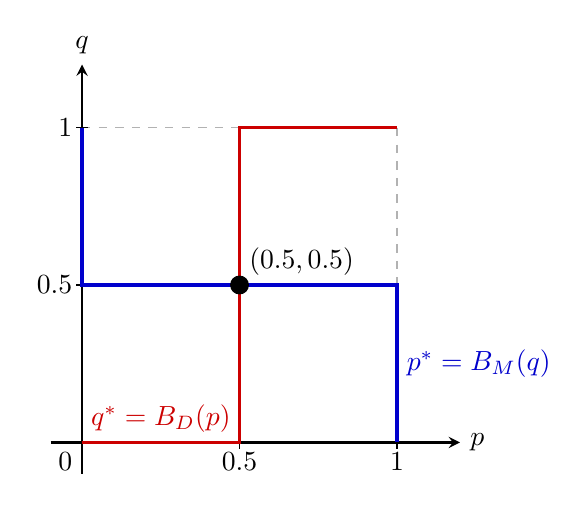
\begin{tikzpicture}[scale=4, >=stealth]
    % Axes
    \draw[->, thick] (-0.1, 0) -- (1.2, 0) node[right] {$p$};
    \draw[->, thick] (0, -0.1) -- (0, 1.2) node[above] {$q$};

    % Unit square bounding box (dashed)
    \draw[dashed, gray!60] (0, 1) -- (1, 1) -- (1, 0);

    % Axis labels/ticks
    \node[below left] at (0, 0) {$0$};
    \node[below] at (0.5, 0) {$0.5$};
    \node[below] at (1, 0) {$1$};
    \node[left] at (0, 0.5) {$0.5$};
    \node[left] at (0, 1) {$1$};

    % Tick marks
    \draw (0.5, 0.02) -- (0.5, -0.02);
    \draw (1, 0.02) -- (1, -0.02);
    \draw (0.02, 0.5) -- (-0.02, 0.5);
    \draw (0.02, 1) -- (-0.02, 1);

    % Best response B_D(p) - Red Line
    % For p < 0.5, q = 0
    % For p = 0.5, q in [0, 1]
    % For p > 0.5, q = 1
    \draw[very thick, red!80!black] (0, 0) -- (0.5, 0) -- (0.5, 1) -- (1, 1);

    % Best response B_M(q) - Blue Line
    % For q < 0.5, p = 1
    % For q = 0.5, p in [0, 1]
    % For q > 0.5, p = 0
    \draw[very thick, blue!80!black] (1, 0) -- (1, 0.5) -- (0, 0.5) -- (0, 1);

    % Nash Equilibrium Point
    \filldraw[black] (0.5, 0.5) circle (0.8pt);
    \node[above right] at (0.5, 0.5) {$(0.5, 0.5)$};

    % Legend / Curve Labels
    \node[blue!80!black, right] at (1, 0.25) {$p^* = B_M(q)$};
    \node[red!80!black, above] at (0.25, 0) {$q^* = B_D(p)$};

\end{tikzpicture}

\end{document}

    }
    \end{figure}

    \item \textbf{Example 2.8. Volunteer's Dilemma.} \(k\) students are in the classroom, where the professor has just said something confusing. Each of the student decides to raise their hand and ask for clarification or not, but doing so is costly:
    \[
    u_i =
    \begin{cases}
        2 &\text{if } i \text{ remains silent but someone else asks for clarification} \\
        1 &\text{if } i \text{ asks for clarification} \\
        0 &\text{if no one asks for clarification}
    \end{cases}
    \]
    \begin{itemize}
        \item There are \(k\) possible pure strategy Nash equilibria where exactly one student asks for clarification, which is unrealistic if students don't know each other well.
        \item We want to find a \textbf{symmetric equilibrium}, where everyone plays the same mixed strategy.
        \item Suppose every other student randomly asks for clarification with the same probability \(p\), what is my best response?
        \[
        \begin{cases}
            U(Y,p) = 1 \\
            U(N,p) = [1-(1-p)^{k-1}] \cdot 2
        \end{cases}
        \]
        \item For me to randomize, these two must be equal (indifferent) in the Nash equilibrium, and the same holds for every other student. Therefore, for every student, the probability of asking for clarification is:
        \[
        p^* = 1-(0.5)^\frac{1}{k-1}
        \]
        \item \(p^*\) decreases with \(k\): The more students, the less likely one asks for clarification.
        \item Probability of no one asking = \((0.5)^\frac{k}{k-1}\), which is increasing with \(k\). The more students, the less likely anyone asks for clarification at all.
        \item Free rider problem: An important concept in the study of public goods.
    \end{itemize}
\end{itemize}

\subsection{Domination}

\begin{itemize}
    \item Recall that in \textit{Prisoner's Dilemma}, we say that defecting is strictly better than cooperating. In other words, cooperating is a \textbf{strictly dominated} action.
    \item \textbf{Definition 2.3.} For player \(i\), an action \(a_i \in A_i\) is \textbf{strictly dominated} by another action \(a_i' \in A_i\) if for any \(\mathbf{a}_{-i} \in \mathbf{A}_{-i}\):
    \[
    U_i(a_i, \mathbf{a}_{-i}) < U_i(a_i', \mathbf{a}_{-i})
    \]
    \item \textbf{Theorem 2.6.} A strictly dominated action is never played in any Nash equilibrium.
    \begin{itemize}
        \item \textit{Proof.} If \(a_i\) is strictly dominated, then \(a_i \notin b_i(\boldsymbol{\sigma}_{-i})\) for any \(\boldsymbol{\sigma}_{-i}\). In a Nash equilibrium \(\boldsymbol{\sigma}^*\), we have \(\sigma_i^* \in B_i(\boldsymbol{\sigma}_{-i})\), and because \(a_i \notin b_i(\boldsymbol{\sigma}_{-i})\), by Theorem 2.4 we must have \(\sigma_i^*(a_i) = 0\).
    \end{itemize}
    \item We can derive a corollary: If a strategy profile is a Nash equilibrium, it remains a Nash equilibrium if we delete every strictly dominated actions.
    \item One use of this is to reduce a game to a \(2 \times 2\) matrix, where we can assign probabilities of \(p\) and \(1-p\), \(q\) and \(1-q\).

    \item Example:
    
    \begin{table}[h]
    \begin{center}
    \begin{tabular}{llccc}
    &&
    \multicolumn{3}{c}{Column} \\&& 
    $C_1$ & 
    $C_2$ & 
    $C_3$
    \\ \cline{3-5} 
    \multirow{3}{*}{Row} & 
    \multicolumn{1}{c|}{$R_1$} & 
    \multicolumn{1}{c|}{(3, 3)} &
    \multicolumn{1}{c|}{(1, 1)} &
    \multicolumn{1}{c|}{(4, 0)}
    \\ \cline{3-5} & 
    \multicolumn{1}{c|}{$R_2$} & 
    \multicolumn{1}{c|}{(2, 1)} &
    \multicolumn{1}{c|}{(3, 4)} &
    \multicolumn{1}{c|}{(1, 2)}
    \\ \cline{3-5} & 
    \multicolumn{1}{c|}{$R_3$}& 
    \multicolumn{1}{c|}{(0, 2)} &
    \multicolumn{1}{c|}{(0, 0)} &
    \multicolumn{1}{c|}{(0, 1)}
    \\ \cline{3-5} 
    \end{tabular}
    \end{center}
    \end{table}
    
    \begin{enumerate}
        \item[\textcolor{blue}{1.}] First, for Row player, we can see that \(R3\) is strictly dominated by both \(R1\) and \(R2\), so we can delete the whole row.
        \item[\textcolor{red}{2.}] Then, in the remaining \(2 \times 3\) game, for Column player, \(C3\) is strictly dominated by \(C2\), so we can delete the whole column.
        \item[3.] We are left with the final \(2 \times 2\) game, which is helpful to find a mixed strategy Nash equilibrium.
    \end{enumerate}

    \begin{table}[h]
    \begin{center}
    \begin{tabular}{llccc}
    &&
    \multicolumn{3}{c}{Column Player} \\&& 
    $C_1$ & 
    $C_2$ & 
    \redstrike{$C_3$}
    \\ \cline{3-5} 
    \multirow{3}{*}{Row Player} & 
    \multicolumn{1}{c|}{$R_1$} & 
    \multicolumn{1}{c|}{(3, 3)} &
    \multicolumn{1}{c|}{(1, 1)} &
    \multicolumn{1}{c|}{\redstrike{(4, 0)}}
    \\ \cline{3-5} & 
    \multicolumn{1}{c|}{$R_2$} & 
    \multicolumn{1}{c|}{(2, 1)} &
    \multicolumn{1}{c|}{(3, 4)} &
    \multicolumn{1}{c|}{\redstrike{(1, 2)}}
    \\ \cline{3-5} & 
    \multicolumn{1}{c|}{\bluestrike{$R_3$}} & 
    \multicolumn{1}{c|}{\bluestrike{(0, 2)}} &
    \multicolumn{1}{c|}{\bluestrike{(0, 0)}} &
    \multicolumn{1}{c|}{\bluestrike{\redstrike{(0, 1)}}}
    \\ \cline{3-5} 
    \end{tabular}
    \end{center}
\end{table}

    \item In some games, including \textit{Prisoner's Dilemma}, the pure strategy Nash equilibrium can be found by \textbf{iterated elimination of strictly dominated strategies (IESDS)} alone. The result is a \textbf{dominant equilibrium}.
    \item \textbf{Example 2.9. Guess \(\frac{2}{3}\) of the Average.} A group of \(n\) players are guessing a real number \(a_i \in [0,100]\). Their goal is to guess as close as the \(\frac{2}{3}\) of the average guess as possible, so:
    \[
    u_i = -\left|a_i - \frac{2}{3}\cdot\frac{\sum^n_{j=1} a_j}{n}\right|
    \]
    \begin{enumerate}
        \item First, we can find that the \(\frac{2}{3}\) of the average must not exceed 66.67. Therefore, any number greater than 66.67 are dominated by 66.67 and can be deleted.
        \item In the remaining choice [0,66.67], the \(\frac{2}{3}\) of the average must not exceed 44.45. Therefore, any number greater than 44.45 are dominated by 44.45 and can be deleted.
        \item As the iteration goes on, the only remaining available number would be 0. Thus, the unique Nash equilibrium is everyone guessing 0.
    \end{enumerate}

\end{itemize}

\section{Dynamic Games and the Subgame Perfect Equilibrium}

\begin{itemize}
    \item We move on to study dynamic games, where players move in turns.
    \item \textbf{Example 3.1. Dynamic Battle of Sexes.} The game setting is similar, except now Adam can make his choice first.
    \begin{enumerate}
        \item Adam's choices: \(\{H, R\}\)
        \item[2.1.] Eve's choices after Adam chooses \(H\): \(\{H, R\}\)
        \item[2.2.] Eve's choices after Adam chooses \(R\): \(\{H, R\}\)
    \end{enumerate}
    \begin{itemize}
    \item Same as the static game, there are four possible outcomes, where each outcome give different utilities to each player.
    \item Instead of using a payoff matrix, we use a \textbf{game tree} to represent the game, also known as an \textbf{extensive-form game}:
    \newpage

    \begin{figure}[h]
    \centering
    \resizebox{0.4\textwidth}{!}{
    \documentclass[tikz,border=5mm]{standalone}
\usepackage{xcolor}

\begin{document}
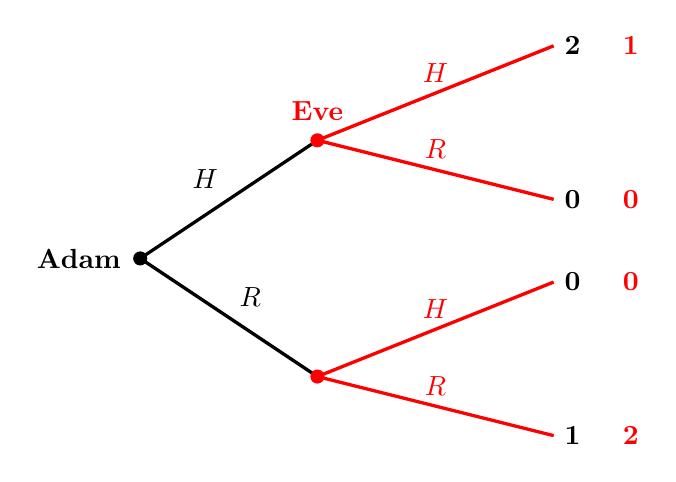
\begin{tikzpicture}[
    scale=1.5,
    font=\bfseries,
    dot/.style={circle, fill=#1, inner sep=1.8pt},
    dot/.default=black,
    line width=1.2pt
]

    % Coordinates
    \coordinate (root) at (0, 0);
    \coordinate (eve_top) at (1.5, 1);
    \coordinate (eve_bot) at (1.5, -1);
    
    \coordinate (leaf1) at (3.5, 1.8);
    \coordinate (leaf2) at (3.5, 0.5);
    \coordinate (leaf3) at (3.5, -0.2);
    \coordinate (leaf4) at (3.5, -1.5);

    % Level 1 branches (Adam)
    \draw[black] (root) -- (eve_top) node[midway, above left] {$H$};
    \draw[black] (root) -- (eve_bot) node[midway, above right] {$R$};

    % Level 2 branches (Eve)
    \draw[red] (eve_top) -- (leaf1) node[midway, above] {$H$};
    \draw[red] (eve_top) -- (leaf2) node[midway, above] {$R$};
    \draw[red] (eve_bot) -- (leaf3) node[midway, above] {$H$};
    \draw[red] (eve_bot) -- (leaf4) node[midway, above] {$R$};

    % Nodes
    \node[dot=black, label=left:Adam] at (root) {};
    \node[dot=red, label={[red]above:Eve}] at (eve_top) {};
    \node[dot=red] at (eve_bot) {};

    % Payoffs
    \node[right] at (leaf1) {2 \quad \textcolor{red}{1}};
    \node[right] at (leaf2) {0 \quad \textcolor{red}{0}};
    \node[right] at (leaf3) {0 \quad \textcolor{red}{0}};
    \node[right] at (leaf4) {1 \quad \textcolor{red}{2}};

\end{tikzpicture}
\end{document}


    }
    \end{figure}
    \end{itemize}

    \item Note that after a player makes a move, the next player doesn't necessarily have the same set of choices, or even need to be the same player.

    \begin{figure}[h]
    \centering
    \resizebox{0.4\textwidth}{!}{
    \documentclass[tikz,border=5mm]{standalone}
\usepackage{xcolor}

\begin{document}
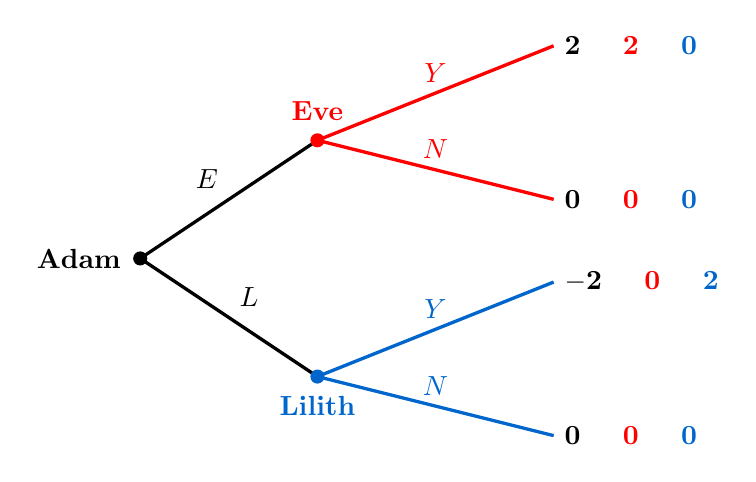
\begin{tikzpicture}[
    scale=1.5,
    font=\bfseries,
    dot/.style={circle, fill=#1, inner sep=1.8pt},
    dot/.default=black,
    line width=1.2pt
]

    % Coordinates
    \coordinate (root)   at (0, 0);
    \coordinate (eve)    at (1.5, 1);
    \coordinate (lilith) at (1.5, -1);
    
    \coordinate (leaf1) at (3.5, 1.8);
    \coordinate (leaf2) at (3.5, 0.5);
    \coordinate (leaf3) at (3.5, -0.2);
    \coordinate (leaf4) at (3.5, -1.5);

    % Level 1 branches (Adam)
    \draw[black] (root) -- (eve)    node[midway, above left] {$E$};
    \draw[black] (root) -- (lilith) node[midway, above right] {$L$};

    % Level 2 branches (Eve - Red)
    \draw[red] (eve) -- (leaf1) node[midway, above] {$Y$};
    \draw[red] (eve) -- (leaf2) node[midway, above] {$N$};

    % Level 2 branches (Lilith - Blue)
    \definecolor{gameblue}{RGB}{0, 102, 204}
    \draw[gameblue] (lilith) -- (leaf3) node[midway, above] {$Y$};
    \draw[gameblue] (lilith) -- (leaf4) node[midway, above] {$N$};

    % Decision Nodes
    \node[dot=black, label=left:Adam] at (root) {};
    \node[dot=red, label={[red]above:Eve}] at (eve) {};
    \node[dot=gameblue, label={[gameblue]below:Lilith}] at (lilith) {};

    % Payoffs (Adam: black, Eve: red, Lilith: blue)
    \node[right] at (leaf1) {2 \quad \textcolor{red}{2} \quad \textcolor{gameblue}{0}};
    \node[right] at (leaf2) {0 \quad \textcolor{red}{0} \quad \textcolor{gameblue}{0}};
    \node[right] at (leaf3) {$-$2 \quad \textcolor{red}{0} \quad \textcolor{gameblue}{2}};
    \node[right] at (leaf4) {0 \quad \textcolor{red}{0} \quad \textcolor{gameblue}{0}};

\end{tikzpicture}
\end{document}

    }
    \end{figure}

    \item To formalize a dynamic game, we introduction \textbf{history}:
    \begin{itemize}
        \item A history \(h\) is a node on the game tree, which corresponds to a sequence of actions previously taken.
        \item For example, the initial history \(\emptyset\), an intermediate history \((H_A)\), or a terminal (ending) history \((H_A, H_E)\).
        \item The set of all possible histories: \(H\).
        \item The player moving after \(h\): \(\mathbb{P}(h)\).
        \item Actions available moving after \(h\): \(A(h)\).
        \item Utility for player \(i\) after a terminal history \(h\): \(u_i(h)\).
    \end{itemize}

    \item What is a strategy in a dynamic game?
    \begin{itemize}
        \item Instead of one single action or pure strategy, here a strategy is a \textbf{contingent plan}.
    \end{itemize}
    \item A \textbf{pure strategy} for player \(i\) is a contingent plan that specifies an action from \(A(h)\) at every history \(h\) where player \(i\) needs to move.
    \item A \textbf{mixed strategy} is a contingent plan that specifies an action from \(\Delta(A(h))\) at every history \(h\) where player \(i\) needs to move.
    \begin{itemize}
        \item We will discuss pure strategies most of the time.
    \end{itemize}
    \item For example, Eve needs to decide what to play if Adam plays \(H\), as well as that if Adam plays \(R\).
    \item Then, we can put every players' strategies together into a \textbf{strategy profile}. This can be represented on a game tree.

    \newpage
    \begin{figure}[h]
    \centering
    \resizebox{0.4\textwidth}{!}{
    \documentclass[tikz,border=5mm]{standalone}
\usepackage{xcolor}
\usetikzlibrary{shapes.geometric, decorations.markings, arrows.meta}

\definecolor{gamegreen}{RGB}{58, 107, 34}

\begin{document}
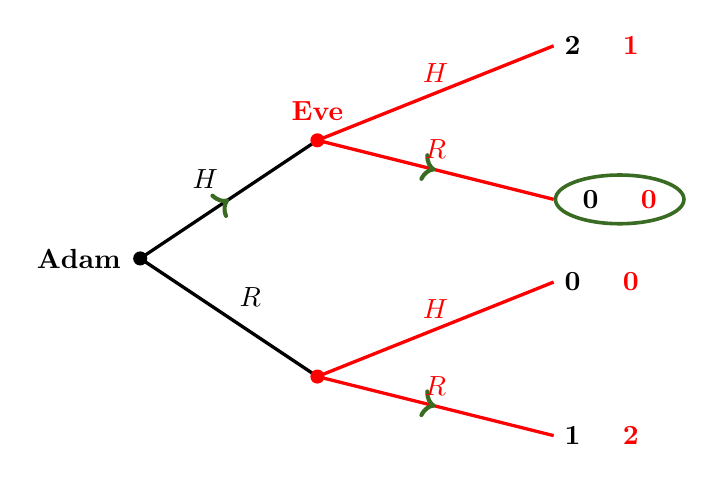
\begin{tikzpicture}[
    scale=1.5,
    font=\bfseries,
    dot/.style={circle, fill=#1, inner sep=1.8pt},
    dot/.default=black,
    line width=1.2pt,
    % Style to put a green arrow along the branch
    green arrow/.style={
        postaction={
            decorate,
            decoration={
                markings,
                mark=at position 0.5 with {
                    \arrow[gamegreen, line width=1.5pt]{>};
                }
            }
        }
    }
]

    % Coordinates
    \coordinate (root) at (0, 0);
    \coordinate (eve_top) at (1.5, 1);
    \coordinate (eve_bot) at (1.5, -1);
    
    \coordinate (leaf1) at (3.5, 1.8);
    \coordinate (leaf2) at (3.5, 0.5);
    \coordinate (leaf3) at (3.5, -0.2);
    \coordinate (leaf4) at (3.5, -1.5);

    % Level 1 branches (Adam)
    \draw[black, green arrow] (root) -- (eve_top) node[midway, above left] {$H$};
    \draw[black] (root) -- (eve_bot) node[midway, above right] {$R$};

    % Level 2 branches (Eve)
    \draw[red] (eve_top) -- (leaf1) node[midway, above] {$H$};
    \draw[red, green arrow] (eve_top) -- (leaf2) node[midway, above] {$R$};
    
    \draw[red] (eve_bot) -- (leaf3) node[midway, above] {$H$};
    \draw[red, green arrow] (eve_bot) -- (leaf4) node[midway, above] {$R$};

    % Decision Nodes
    \node[dot=black, label=left:Adam] at (root) {};
    \node[dot=red, label={[red]above:Eve}] at (eve_top) {};
    \node[dot=red] at (eve_bot) {};

    % Payoffs
    \node[right] at (leaf1) {2 \quad \textcolor{red}{1}};
    \node[right, draw=gamegreen, ellipse, line width=1.3pt, inner sep=3pt] at (leaf2) {0 \quad \textcolor{red}{0}};
    \node[right] at (leaf3) {0 \quad \textcolor{red}{0}};
    \node[right] at (leaf4) {1 \quad \textcolor{red}{2}};

\end{tikzpicture}
\end{document}
    }
    \end{figure}

    \item Will this strategy profile will realize?
    \begin{itemize}
        \item Nash equilibrium: Is there any profitable deviation?
    \end{itemize}
    \item Not Nash equilibrium:
    \begin{itemize}
        \item Adam can deviate to \(A_A(\emptyset) = R\) instead of \(H\): \(U_A(R,\textcolor{red}{R}) = 1 > 0 = U_A(H,\textcolor{red}{R})\).
        \item Eve can deviate to \(A_E(H) = \textcolor{red}{H}\) instead of \(\textcolor{red}{R}\): \(U_E(H,\textcolor{red}{H}) = 1 > 0 = U_E(H,\textcolor{red}{R})\).
    \end{itemize}
    \item Consider another strategy profile: 
    \begin{figure}[h]
    \centering
    \resizebox{0.4\textwidth}{!}{
    \input{stubborneve2}
    }
    \end{figure}

    \item This is a Nash equilibrium: No profitable deviation.
    \item But looking closer, at the top right subtree, Eve decides to play \(R\) if Adam plays \(H\), which is not something a rational player would do.
    \begin{itemize}
        \item We call this a \textbf{non-credible threat}.
    \end{itemize}
    \item Even if something doesn't happen at the end, we still want the contingent plan to be rational and optimizing.
    \item If we see the subtree as a game itself (a \textbf{subgame}), then we want all of the subgames to be optimal, i.e. no profitable deviation.
    \item \textbf{Definition 3.1.} A strategy profile \(\mathbf{s}\) is a \textbf{subgame perfect equilibrium (SPE)} if there is no profitable deviation for any player in any subgame.
    \item How to find an SPE in practice?
    \begin{itemize}
        \item \textbf{Backward induction}.
    \end{itemize}
    \begin{enumerate}
        \item For the last player(s), find their best actions they can make in each node.
        \item Knowing what the last player will do, find the best actions the second last player can do.
        \item Repeat until the first player.
    \end{enumerate}
    \item For example,
    \begin{itemize}
        \item Eve must choose \(H\) if Adam chooses \(H\), and \(R\) if Adam chooses \(R\).
        \item Knowing this, Adam must choose \(H\).
    \end{itemize}
    \item \textbf{Theorem 3.1.} A strategy profile is a subgame perfect equilibrium if and only if it can be obtained by backward induction.
    \item \textbf{Example 3.2. Asking for Extra Credit (Chain Store Paradox).} \(n\) students decide whether to go to the professor's office to appeal their exam scores, and the professor decides whether to comply if a student appeals. The students want higher scores, but staying away is better than going and receiving no extra points. The professor prefers that students do not come, but if they do, complying is easier than refusing.

    \begin{itemize}
        \item We start with a 1-student case.
        
        \begin{figure}[h]
        \centering
        \resizebox{0.4\textwidth}{!}{
        \documentclass[tikz,border=5mm]{standalone}
\usepackage{xcolor}

\begin{document}
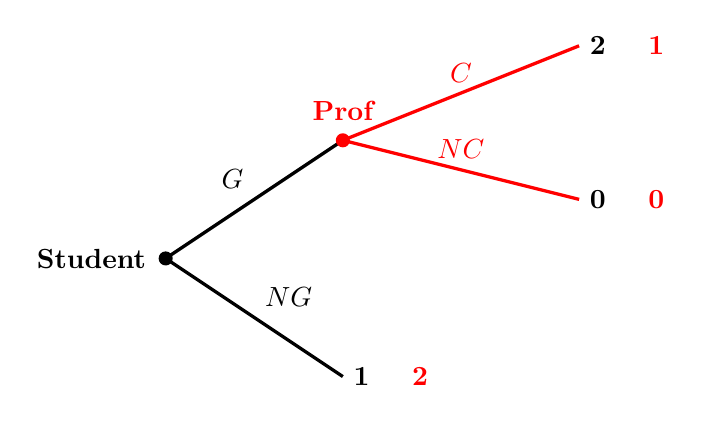
\begin{tikzpicture}[
    scale=1.5,
    font=\bfseries,
    dot/.style={circle, fill=#1, inner sep=1.8pt},
    dot/.default=black,
    line width=1.2pt
]

    % Coordinates
    \coordinate (root) at (0, 0);
    \coordinate (eve_top) at (1.5, 1);
    \coordinate (eve_bot) at (1.5, -1);
    
    \coordinate (leaf1) at (3.5, 1.8);
    \coordinate (leaf2) at (3.5, 0.5);

    % Level 1 branches (Adam)
    \draw[black] (root) -- (eve_top) node[midway, above left] {$G$};
    \draw[black] (root) -- (eve_bot) node[midway, above right] {$NG$};

    % Level 2 branches (Eve)
    \draw[red] (eve_top) -- (leaf1) node[midway, above] {$C$};
    \draw[red] (eve_top) -- (leaf2) node[midway, above] {$NC$};

    % Nodes
    \node[dot=black, label=left:Student] at (root) {};
    \node[dot=red, label={[red]above:Prof}] at (eve_top) {};

    % Payoffs
    \node[right] at (eve_bot) {1 \quad \textcolor{red}{2}};
    \node[right] at (leaf1) {2 \quad \textcolor{red}{1}};
    \node[right] at (leaf2) {0 \quad \textcolor{red}{0}};
    
\end{tikzpicture}
\end{document}
        }
        \end{figure}

        \begin{enumerate}
            \item If the student comes, the professor must choose to comply.
            \item Knowing this, the student must choose to go than not going.
        \end{enumerate}

        \item If we extend this to \(n\) students coming one by one, the unique SPE is every student going and the professor complying with everyone.
        \item The \textbf{chain store paradox}: Why do new companies keep entering, and why don't incumbents start a price war?
        \end{itemize}

    \item \textbf{Example 3.3. Centipede Game.} Two players, \(A\) and \(B\), choose to either stop and keep 80\% of the jackpot, or double it and pass to the other player to choose.

    \begin{figure}[h]
    \centering
    \resizebox{0.7\textwidth}{!}{
    
\documentclass[tikz,border=5mm]{standalone}
\usepackage{xcolor}

\begin{document}
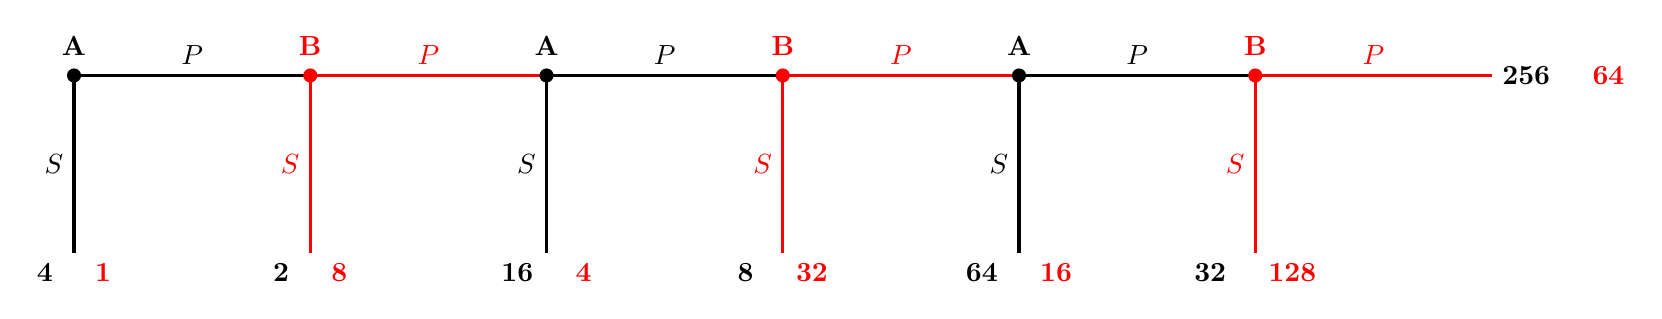
\begin{tikzpicture}[
    scale=1.5,
    font=\bfseries,
    dot/.style={circle, fill=#1, inner sep=1.8pt},
    dot/.default=black,
    line width=1.2pt
]

    % Nodes coordinates
    \coordinate (n1) at (0, 0);
    \coordinate (n2) at (2, 0);
    \coordinate (n3) at (4, 0);
    \coordinate (n4) at (6, 0);
    \coordinate (n5) at (8, 0);
    \coordinate (n6) at (10, 0);
    \coordinate (end) at (12, 0);

    % Downward payoffs coordinates
    \coordinate (d1) at (0, -1.5);
    \coordinate (d2) at (2, -1.5);
    \coordinate (d3) at (4, -1.5);
    \coordinate (d4) at (6, -1.5);
    \coordinate (d5) at (8, -1.5);
    \coordinate (d6) at (10, -1.5);

    % Horizontal branches (Continue / P)
    \draw[black] (n1) -- (n2) node[midway, above] {$P$};
    \draw[red]   (n2) -- (n3) node[midway, above] {$P$};
    \draw[black] (n3) -- (n4) node[midway, above] {$P$};
    \draw[red]   (n4) -- (n5) node[midway, above] {$P$};
    \draw[black] (n5) -- (n6) node[midway, above] {$P$};
    \draw[red]   (n6) -- (end) node[midway, above] {$P$};

    % Downward branches (Stop / S)
    \draw[black] (n1) -- (d1) node[midway, left] {$S$};
    \draw[red]   (n2) -- (d2) node[midway, left] {$S$};
    \draw[black] (n3) -- (d3) node[midway, left] {$S$};
    \draw[red]   (n4) -- (d4) node[midway, left] {$S$};
    \draw[black] (n5) -- (d5) node[midway, left] {$S$};
    \draw[red]   (n6) -- (d6) node[midway, left] {$S$};

    % Decision Nodes & Player Labels
    \node[dot=black, label=above:A] at (n1) {};
    \node[dot=red, label={[red]above:B}] at (n2) {};
    \node[dot=black, label=above:A] at (n3) {};
    \node[dot=red, label={[red]above:B}] at (n4) {};
    \node[dot=black, label=above:A] at (n5) {};
    \node[dot=red, label={[red]above:B}] at (n6) {};

    % Payoffs (A in black, B in red)
    \node[below] at (d1) {4 \quad \textcolor{red}{1}};
    \node[below] at (d2) {2 \quad \textcolor{red}{8}};
    \node[below] at (d3) {16 \quad \textcolor{red}{4}};
    \node[below] at (d4) {8 \quad \textcolor{red}{32}};
    \node[below] at (d5) {64 \quad \textcolor{red}{16}};
    \node[below] at (d6) {32 \quad \textcolor{red}{128}};
    \node[right] at (end) {256 \quad \textcolor{red}{64}};

\end{tikzpicture}
\end{document}


    }
    \end{figure}

    \begin{enumerate}
        \item In the final round, \(B\) must stop and keep most of the money.
        \item In the second last round, \(A\) knows \(B\) must choose to stop after them. Not wanting this to happen, they must stop there instead of passing it down.
        \item The same goes until the beginning: the SPE is \(A\) stopping at the very beginning, giving both players the minimal payoff.
    \end{enumerate}

    \item Sometimes we don't need to have two or more players, but a single player in different stages.

    \item \textbf{Example 3.4. Self-control Game.} A player decides to go to a burger place or a salad place. They can order either burger or salad in the burger place, whereas they can only order salad in a salad place. They prefer to eat salad right now, but if they see a burger later, they will be tempted to order one.

    \newpage
    \begin{figure}[h]
    \centering
    \resizebox{0.4\textwidth}{!}{
    \documentclass[tikz,border=5mm]{standalone}
\usepackage{xcolor}

\begin{document}
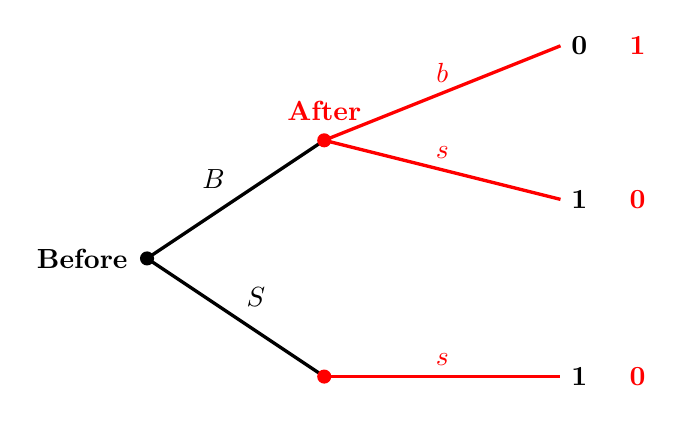
\begin{tikzpicture}[
    scale=1.5,
    font=\bfseries,
    dot/.style={circle, fill=#1, inner sep=1.8pt},
    dot/.default=black,
    line width=1.2pt
]

    % Coordinates
    \coordinate (root)      at (0, 0);
    \coordinate (after_top) at (1.5, 1);
    \coordinate (after_bot) at (1.5, -1);
    
    \coordinate (leaf1) at (3.5, 1.8);
    \coordinate (leaf2) at (3.5, 0.5);
    \coordinate (leaf3) at (3.5, -1);

    % Level 1 branches (Before)
    \draw[black] (root) -- (after_top) node[midway, above left] {$B$};
    \draw[black] (root) -- (after_bot) node[midway, above right] {$S$};

    % Level 2 branches (After)
    \draw[red] (after_top) -- (leaf1) node[midway, above] {$b$};
    \draw[red] (after_top) -- (leaf2) node[midway, above] {$s$};
    \draw[red] (after_bot) -- (leaf3) node[midway, above] {$s$};

    % Decision Nodes & Player Labels
    \node[dot=black, label=left:Before] at (root) {};
    \node[dot=red, label={[red]above:After}] at (after_top) {};
    \node[dot=red] at (after_bot) {};

    % Payoffs (Before: black, After: red)
    \node[right] at (leaf1) {0 \quad \textcolor{red}{1}};
    \node[right] at (leaf2) {1 \quad \textcolor{red}{0}};
    \node[right] at (leaf3) {1 \quad \textcolor{red}{0}};

\end{tikzpicture}
\end{document}

    }
    \end{figure}

    \begin{itemize}
        \item SPE: Go to salad place now.
        \item This is called a \textbf{commitment device}.
    \end{itemize}

    \item Of course, we can study games with continuous choices as well.

    \item \textbf{Example 3.5. Ultimatum Game.} Player 1 proposes how to split \$100 dollars: \((x, 100-x)\). Player 2 chooses to accept or not; if they accept, split accordingly, otherwise, the money is gone, and furthermore, Player 2 is fined with \$1 for rejecting.

    \begin{figure}[h]
    \centering
    \resizebox{0.4\textwidth}{!}{
    \documentclass[tikz,border=5mm]{standalone}
\usepackage{xcolor}

\begin{document}
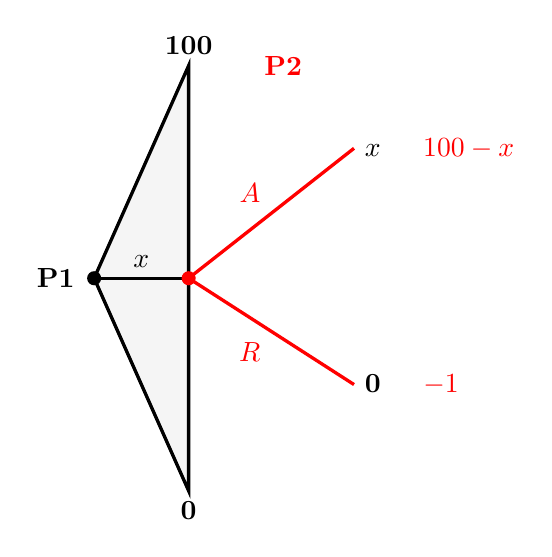
\begin{tikzpicture}[
    scale=1.5,
    font=\bfseries,
    dot/.style={circle, fill=#1, inner sep=1.8pt},
    dot/.default=black,
    line width=1.2pt
]

    % Coordinates
    \coordinate (p1)   at (0, 0);
    \coordinate (top)  at (0.8, 1.8);
    \coordinate (mid)  at (0.8, 0);
    \coordinate (bot)  at (0.8, -1.8);

    \coordinate (leaf_top) at (2.2, 1.1);
    \coordinate (leaf_bot) at (2.2, -0.9);

    % Player 1 continuous action wedge/arc
    \draw[black, fill=gray!8] (p1) -- (top) -- (bot) -- cycle;
    \draw[black] (p1) -- (mid) node[midway, above] {$x$};

    % Continuum labels for Player 1
    \node[above] at (top) {100};
    \node[below] at (bot) {0};

    % Player 2 branches (Red)
    \draw[red] (mid) -- (leaf_top) node[midway, above left] {$A$};
    \draw[red] (mid) -- (leaf_bot) node[midway, below left] {$R$};

    % Nodes & Player labels
    \node[dot=black, label=left:P1] at (p1) {};
    \node[dot=red] at (mid) {};
    \node[red] at (1.6, 1.8) {P2};

    % Payoffs (P1: black, P2: red)
    \node[right] at (leaf_top) {$x$ \quad \textcolor{red}{$100 - x$}};
    \node[right] at (leaf_bot) {0 \quad \textcolor{red}{$-1$}};

\end{tikzpicture}
\end{document}

    }
    \end{figure}

    \begin{enumerate}
        \item Since \(100-x > -1\) for all \(x \in [0,100]\), Player 2 must accept no matter what \(x\) is.
        \item Knowing this, Player 1 must maximize. The SPE is \(x = 100\) and Player 2 accepts: Player 1 keeps all the money.
    \end{enumerate}
    
\end{itemize}

\section{Static Games with Incomplete Information and the Bayes Nash Equilibrium}

\begin{itemize}
    \item In all previous models, players' strategies depends on the fact that they know exactly about the opponent(s).
    \item What if they don't know who they are playing against?
    \item \textbf{Example 4.1. Battle of Sexes with Incomplete Information.} Suppose Eve can be one of the two ``types" with probability \(p\), but Adam doesn't know which type of Eve he is playing against, then we have two possible games:

    \newpage
    \begin{table}[h]
    \centering
    \begin{tabular}{llcc}
    &&
    \multicolumn{2}{c}{\textcolor{blue}{Eve}}  \\&& 
    \textcolor{blue}{Horror} & 
    \textcolor{blue}{Romance} 
    \\ \cline{3-4} 
    \multirow{2}{*}{\textcolor{red}{Adam}} & 
    \multicolumn{1}{c|}{\textcolor{red}{Horror}} & 
    \multicolumn{1}{c|}{(\textcolor{red}{2}, \textcolor{blue}{1})} &
    \multicolumn{1}{c|}{(\textcolor{red}{0}, \textcolor{blue}{0})} 
    \\ \cline{3-4} & 
    \multicolumn{1}{c|}{\textcolor{red}{Romance}} & 
    \multicolumn{1}{c|}{(\textcolor{red}{0}, \textcolor{blue}{0})} &
    \multicolumn{1}{c|}{(\textcolor{red}{1}, \textcolor{blue}{2})} 
    \\ \cline{3-4}
    \multicolumn{4}{c}{} \\
    \multicolumn{4}{c}{``Normal" Eve}
    \end{tabular}
    \end{table}

    \begin{table}[h]
    \centering
    \begin{tabular}{llcc}
    &&
    \multicolumn{2}{c}{\textcolor{blue}{Eve}}  \\&& 
    \textcolor{blue}{Horror} & 
    \textcolor{blue}{Romance} 
    \\ \cline{3-4} 
    \multirow{2}{*}{\textcolor{red}{Adam}} & 
    \multicolumn{1}{c|}{\textcolor{red}{Horror}} & 
    \multicolumn{1}{c|}{(\textcolor{red}{2}, \textcolor{blue}{0})} &
    \multicolumn{1}{c|}{(\textcolor{red}{0}, \textcolor{blue}{1})} 
    \\ \cline{3-4} & 
    \multicolumn{1}{c|}{\textcolor{red}{Romance}} & 
    \multicolumn{1}{c|}{(\textcolor{red}{0}, \textcolor{blue}{2})} &
    \multicolumn{1}{c|}{(\textcolor{red}{1}, \textcolor{blue}{0})} 
    \\ \cline{3-4}
    \multicolumn{4}{c}{} \\
    \multicolumn{4}{c}{``Moody" Eve}
    \end{tabular}
    \end{table}

    \begin{itemize}
        \item Because Eve's type is her \textbf{private information}, she can play her strategy accordingly: \(\sigma_E^N \in \Delta(\{H,R\})\) and \(\sigma_E^M \in \Delta(\{H,R\})\); but because Adam doesn't know, he can only play one strategy: \(\sigma_A \in \Delta(\{H,R\})\).
    \end{itemize}

    \item Formally, in a game with incomplete information:
    \begin{itemize}
        \item Each player \(i\) has a set of \textbf{type}: \(T_i\). For example, \(T_A = \{Normal\}\) and \(T_E = \{Normal, Moody\}\).
        \item \(t_i \in T_i\) is the private information of player \(i\). Other players don't know other players' type, but know the distribution; for example, \(\mathbb{P}(t_E = M) = p\).
        \item Utility depends both the action profile \(\mathbf{a}\) and the type profile \(\mathbf{t}\). For example, \(u_E((H,H)|(n,n)) = 1\), \(u_E((H,H)|(n,m)) = 0\).
        \item A strategy profile specifies a mixed strategy for every type of player. For example, \((\sigma_A, \sigma_E^N, \sigma_E^M)\).
    \end{itemize}

    \item How do players make decisions?
    \begin{itemize}
        \item Because we're dealing with probabilities, players maximizing \textbf{expected utility} will return to the traditional definition of expected values.
        \item For example, we will frequently use the law of total expectation: \[U(\textbf{a}) = \mathbb{E}(u(\textbf{a})) = \mathbb{E}(\mathbb{E}(u(\textbf{a}) \mid \mathbf{t})) = \sum_j \mathbb{P}(\mathbf{t} = \mathbf{t}_j)\mathbb{E}(u(\textbf{a}\mid \mathbf{t} = \mathbf{t}_j)) \]
    \end{itemize}

    \item \textbf{Definition 4.1.} A \textbf{Bayes Nash equilibrium (BNE)} is a strategy profile such that there is no profitable deviation for every type of any player.

    \item Consider the pure strategy profile: \(a_A = H, a_E^N = H, a_E^M = R\).
    \begin{itemize}
        \item Clearly both types of Eve have no incentive to deviate.
        \item For Adam,
        \[
        \begin{cases}
            U_A(H) = 2(1-p) + 0p = 2-2p \\
            U_A(R) = 0(1-p) + 1p = p
        \end{cases}
        \]
        \item Therefore, Adam has no profitable deviation if \(2-2p \ge p\). If \(p \le \frac{2}{3}\), this pure strategy profile is a BNE.
        \item Intuition: If Eve is less likely to be Moody, Adam is safe to choose Horror.
    \end{itemize}
    \item When more players have more than one possible type, the \textbf{probability distribution} becomes important.
    \item \textbf{Example 4.2. Battle of Sexes with Joint Distribution.} Suppose now Adam can also be moody, and the utility for both players are given by the follows:
    \[
    \begin{cases}
        \text{Watching preferred movie alone} & \text{: 0 if normal, 2 if moody} \\ 
        \text{Watching less preferred movie alone} & \text{: 0 if normal, 1 if moody} \\ 
        \text{Watching preferred movie with company} & \text{: 2 if normal, 0 if moody} \\ 
        \text{Watching less preferred movie with company} & \text{: 1 if normal, 0 if moody} \\ 
    \end{cases}
    \]
    %\newpage
    Furthermore, the joint probability distribution of types is given by:
    \begin{table}[h]
    \centering
    \begin{tabular}{llcc}
    &&
    \multicolumn{2}{c}{Eve}  \\&& 
    Normal & 
    Moody
    \\ \cline{3-4} 
    \multirow{2}{*}{Adam} & 
    \multicolumn{1}{c|}{Normal} & 
    \multicolumn{1}{c|}{0.5} &
    \multicolumn{1}{c|}{0.1} 
    \\ \cline{3-4} & 
    \multicolumn{1}{c|}{Moody} & 
    \multicolumn{1}{c|}{0.1} &
    \multicolumn{1}{c|}{0.3} 
    \\ \cline{3-4}
    \end{tabular}
    \end{table}

    \begin{itemize}
        \item How does each player determine their opponent?
        \item To us, Eve is normal with probability \(0.5+0.1=0.6\).
        \item But to the players, they rely on their \textbf{posterior belief}.
        \item For example, to Normal Adam,
        \[
        \mathbb{P}(t_E = N | t_A = N) = \frac{\mathbb{P}(t_E = N, t_A = N)}{\mathbb{P}(t_A = N)} = \frac{0.5}{0.5+0.1} = \frac{5}{6}
        \]
        \item To check if a strategy profile is a BNE, we simply check for every type of every player whether there is any profitable deviation.
        \item Consider the pure strategy profile where Normal Adam, Moody Adam and Normal Eve play H, and Moody Eve plays R.
        \item For Normal Adam,
        \[
        \begin{cases}
            U_A^N(H) = \frac{5}{6} \cdot 2 + \frac{1}{6} \cdot 0 = \frac{5}{3} \\
            U_A^N(R) = \frac{5}{6} \cdot 0 + \frac{1}{6} \cdot 1 = \frac{1}{6}
        \end{cases}
        \]
        \item One can verify that all types of players have no profitable deviation, so this is a BNE.
    \end{itemize}

    \item One of the most common use of the model is \textbf{auction}, where each player's valuation for the goods can be viewed as their private information, i.e. type.

    \item \textbf{Example 4.3. Sealed-bid auction.} A house is being auctioned off. \(n\) players are interested, and each of them has their own valuation \(t_i\) for the house. Given a final price \(p\), their utility is given by:
    \[
    u_i = 
    \begin{cases}
        t_i-p & \text{if } i \text{ wins} \\
        0 & \text{otherwise}
    \end{cases}
    \]
    \begin{itemize}
        \item \textit{Remark.} For simplicity, suppose there is no ties. In fact, most of the time, we will find that ties do not happen at all because we assume a continuous distribution, where \(\mathbb{P}(t_i=x)=0\).
        \item How to determine who wins?
        \item For a static game, we use a \textbf{sealed-bid auction}, where everyone submits a bid \(a_i \in \mathbb{R}^+\) at once and the highest bidder wins.
        \item How much does the winner, bidder \(i\), pay?
        \item First price (highest bid): \(p=a_i\), Second price (second highest bid): \(p=\max_{j\ne i}a_j\)...
        \item To make the auction ``fair", we naturally want everyone's bid to reflect their true valuation in the equilibrium. That's why we study \textbf{mechanism design}.
    \end{itemize}
    \item \textbf{Example 4.3.1. Sealed-bid Second-price Auction.}
    \begin{itemize}
        \item For a second-price auction, we claim that everyone bidding their own type is a BNE.
        \item Showing this is simple: We can show that bidding one's own type is always weakly better, i.e. a best strategy, regardless of other bidders' valuations or bids.
        \item In other words: Will bidder \(i\) be better off in any cases if they don't truthfully report, i.e. \(a_i \ne t_i\)?
        \item Let \(a_{-i} = \max_{j\ne i}a_j\) be the highest competing bid. Note that this is the only other bid we need to concern, and the utility function is:
        \[
        u_i = 
        \begin{cases}
            t_i - a_{-i} & \text{if } a_i > a_{-i} \\
            0 & \text{otherwise}
        \end{cases}
        \]
        \item Consider underbidding (\(a_i < t_i\)):
        \begin{enumerate}
            \item \(a_{-i} < a_i\): Bidder \(i\) wins the auction under both strategies. Payoff = \(t_i - a_{-i}\).
            \item \(a_i < a_{-i} < t_i\): Bidder \(i\) loses the auction and their payoff is 0. However, if they truthfully bids \(t_i\) instead, they can win and their payoff can be increased to \(t_i - a_{-i} > 0\).
            \item \(a_{-i} > t_i\): Bidder \(i\) loses the auction under both strategies. Payoff = \(0\).
        \end{enumerate}
        \item Consider overbidding (\(a_i > t_i\)):
        \begin{enumerate}
            \item \(a_{-i} < t_i\): Bidder \(i\) wins the auction under both strategies. Payoff = \(t_i - a_{-i}\).
            \item \(t_i < a_{-i} < a_i\): Bidder \(i\) win the auction and their payoff is \(t_i - a_{-i} < 0\). However, if they truthfully bids \(t_i\) instead, they can lose and their payoff can be increased to \(0\).
            \item \(a_{-i} > a_i\): Bidder \(i\) loses the auction under both strategies. Payoff = \(0\).
        \end{enumerate}
        \item As truthfully bidding is always a best response, everyone doing so is a BNE.
    \end{itemize}

    \item An alternative proof:
    \begin{itemize}
        \item Consider the following cases:
    \begin{enumerate}
        \item \(a_{-i} < t_i\): As \(t_i - a_{-i} > 0\), \(u_i\) is maximized when Bidder \(i\) wins the auction, i.e. bidding \(a_i > a_{-i}\). As \(t_i > a_{-i}\), bidding \(a_i = t_i\) is a best response.
        \item \(a_{-i} > t_i\): As \(t_i - a_{-i} < 0\), \(u_i\) is maximized when Bidder \(i\) loses the auction, i.e. bidding \(a_i < a_{-i}\). As \(t_i < a_{-i}\), bidding \(a_i = t_i\) is a best response.
        \item \(a_{-i} = t_i\): Although we didn't formalize a tie-breaking rule, it is easy to see that the payoff is always 0 in this case, so any bid is a best response.
        \end{enumerate}
        \item As \(a_i = t_i\) is a best response in every cases, everyone bidding truthfully is a BNE.
    \end{itemize}
    
    \item \textbf{Example 4.3.2. Sealed-bid First-price Auction.}
    \begin{itemize}
        \item In a first-price auction, bidding one's own type is not necessarily a best strategy. For example, if one wins the auction by bidding \(a_i = t_i\), it is possible that they lower their bid a bit and still win while paying less.
        \item For simplicity, we study a case where there are only two bidders, where \(t_1, t_2 \overset{\mathrm{i.i.d.}}{\sim}\text{Uniform}(0,1)\).
        \item The utility function is:
        \[
        u_i = 
        \begin{cases}
            t_i - a_i & \text{if } a_i > a_{-i} \\
            0 & \text{otherwise}
        \end{cases}
        \]
        \item We claim that bidding \underline{half} of their types, \(a_i = \frac{t_i}{2}\), is a BNE.
        \item We start from the perspective of Bidder 1. We want to show that bidding \(a_1 = \frac{t_1}{2}\) is a best response against \(a_2 = \frac{t_2}{2}\), that is, their expected utility is maximized this way.
        \item Note that since \(t_2\) is at most 1, \(a_2\) is at most \(\frac{1}{2}\), so Bidder 1 only needs to consider \(a_1 \in [0,\frac{1}{2}]\).
        \item We first find the probability of winning:
        \[
        \mathbb{P}(a_1 > a_2) = \mathbb{P}(a_1 > \frac{t_2}{2}) = \mathbb{P}(t_2 < 2a_1)
        \]
        \item Since \(t_2 \sim \text{Uniform}(0,1)\) and \(2a_1 \in [0,1]\), we have \(\mathbb{P}(t_2 < 2a_1) = 2a_1\).
        \item The expected utility is therefore:
        \[
        U_1 = 2a_1 \cdot (t_1 - a_1)
        \]
        Taking first order condition:
        \begin{align*}
            \frac{\partial U_1}{\partial a_1} = 2t_1 - 4a_1 &= 0 \\
            a_1^* &= \frac{t_1}{2}
        \end{align*}
        \item By symmetry and intersection, a BNE is therefore \((a_1^*, a_2^*) = (\frac{t_1}{2}, \frac{t_2}{2})\).
    \end{itemize}
    \item While both types of auction guarantee the bidder with the highest valuation can win, which one can generate higher revenue for the seller?
    \begin{itemize}
        \item \textbf{Revenue Equivalence Theorem}: Any auction mechanism yield the same expected revenue under risk neutrality and i.i.d. valuations.
    \end{itemize}
    \item For example, in a two-player, \(t_1, t_2 \overset{\mathrm{i.i.d.}}{\sim}\text{Uniform}(0,1)\) setting:
    \item In a second-price auction, \(p=\min\{t_1,t_2\}\). Then, 
    \[
    \mathbb{P}(\min\{t_1,t_2\}>x) = \mathbb{P}(t_1 > x) \cdot \mathbb{P}(t_2 > x) = (1-x)^2
    \]
    By the tail sum formula, we have the expected revenue:
    \[
    \mathbb{E}[\min\{t_1,t_2\}] = \int_0^1\mathbb{P}(\min\{t_1,t_2\}>x)dx = \int_0^1(1-x)^2dx = \frac{1}{3}
    \]
    \item In a first-price auction, \(p = \max\{\frac{t_1}{2},\frac{t_2}{2}\} = \frac{1}{2}\max\{t_1,t_2\}\). Then,
    \[
    \mathbb{P}(\max\{t_1,t_2\}<x) = \mathbb{P}(t_1 < x) \cdot \mathbb{P}(t_2 < x) = x^2
    \]
    By the tail sum formula, we have the expected revenue:
    \[
    \mathbb{E}[\frac{1}{2}\max\{t_1,t_2\}] = \frac{1}{2}\int_0^1\mathbb{P}(\max\{t_1,t_2\}>x)dx = \frac{1}{2}\int_0^1 (1-x^2) dx = \frac{1}{3}
    \]
    \item In the previous example, valuation is \underline{subjective} to each bidder. What if the goods have an \underline{objective} value, and each bidder only knows a part of it?
    \item \textbf{Example 4.4. Common Value Auction.} Two clubs, 1 and 2, scout the same young footballer. They observe the mental and physical qualities of the footballer, \(t_1, t_2 \overset{\mathrm{i.i.d.}}{\sim}\text{Uniform}(0,1)\), respectively, and the footballer's true value is \(v=t_1+t_2\). Both of them take part in a first-price auction, and the utility function is:
    \[
    u_i =
    \begin{cases}
        t_1 + t_2 - a_i & \text{if } a_i > a_{-i} \\
        0 & \text{otherwise}
    \end{cases}
    \]
    \begin{itemize}
        \item We claim that both bidding their own type \(a_i = t_i\) is a BNE.
        \item From the perspective of Bidder 1, suppose Bidder 2 bids \(a_2 = t_2\). Since \(a_2 = t_2 \le 1\), Bidder 1 only needs to consider \(a_1 \in [0,1]\) to win. Then, the probability of winning is:
        \[
        \mathbb{P}(a_1 > a_2) = \mathbb{P}(t_2 < a_1)
        \]
        Since \(t_2 \sim \text{Uniform}(0,1)\) and \(a_1 \in [0,1]\), we have \(\mathbb{P}(t_2 < a_1) = a_1\).
        %\item To compute expected utility, we first need to find an expectation conditional on winning:
        %\[
        %\mathbb{E}[t_2 \mid t_2 < a_1] = \frac{a_1}{2}
        %\]
        \item The expected payoff is then:
        \begin{align*}
            U_1 &= \mathbb{P}(t_2 < a_1) \cdot \mathbb{E}[t_1 + t_2 - a_1 \mid t_2 < a_1] \\
            &= \mathbb{P}(t_2 < a_1) \cdot (\mathbb{E}[t_1 \mid t_2 < a_1] + \mathbb{E}[t_2 \mid t_2 < a_1] - \mathbb{E}[a_1 \mid t_2 < a_1]) \\
            &= a_1 \cdot (t_1 + \frac{a_1}{2} - a_1) \\
            &= a_1t_1 - \frac{a_1^2}{2}
        \end{align*}
        \item Taking first order condition:
        \begin{align*}
            \frac{\partial U_1}{\partial a_1} = t_1 - a_1 &= 0 \\
            a_1^* &= t_1
        \end{align*}
        \item By symmetry and intersection, a BNE is therefore \((a_1^*, a_2^*) = (t_1, t_2)\).
        \item An alternative graphical approach to get the expected utility:
        \begin{figure}[h]
        \centering
        \resizebox{0.35\textwidth}{!}{
        \documentclass[border=10pt]{standalone}
\usepackage{tikz}

\begin{document}
\begin{tikzpicture}
    % Axes with arrows
    \draw[->, thick] (0,0) -- (3,0) node[right] {$t_2$};
    \draw[->, thick] (0,0) -- (0,3) node[above left] {$u_1$};

    % Axis Labels (t1 - a1 and a1)
    \node[left, xshift=-1mm] at (0, 0.8) {$t_1 - a_1$};
    \node[below] at (2.2, 0) {$a_1$};

    % The linear line segment with label to the right
    \draw[thick] (0, 0.8) -- (2.2, 1.8) node[right, xshift=2pt] {$t_1 + t_2 - a_1$};

    % Dashed line
    \draw[dashed, thick] (2.2, 0) -- (2.2, 1.8);

\end{tikzpicture}
\end{document}

        }
        \end{figure}
        
        Hence,
        \[
        U_1 = \int_0^{a_1}t_1+t_2-a_1dt_2 = a_1t_1 - \frac{a_1^2}{2}
        \]
    \end{itemize}
    \item Suppose \(t_1 = x\), then at the beginning, the expected value of the footballer is:
    \[
    \mathbb{E}[t_1+t_2\mid t_1=x] = \mathbb{E}[t_1 \mid t_1=x] + \mathbb{E}[t_2\mid t_1=x] = x + 0.5
    \]
    However, if Bidder \(1\) wins, the expected value becomes:
    \[
    \mathbb{E}[t_1+t_2\mid t_1=x, t_2 < x] = \mathbb{E}[t_1 \mid t_1=x, t_2 < x] + \mathbb{E}[t_2\mid t_1=x, t_2 < x] = x + 0.5x \le x + 0.5
    \]
    which implies winning is a bad news.
    \begin{itemize}
        \item \textbf{Winner's curse}: You winning means that your competitors have more negative information than you do, so they have lower valuations. This is an example of \textbf{adverse selection}.
    \end{itemize}
\end{itemize}

\section{Dynamic Games with Imperfect/Incomplete Information and the Perfect Bayesian Equilibrium}

\subsection{Imperfect Information}
\begin{itemize}
    \item \textbf{Example 5.1. Asking for Extra Credit Extended.} Suppose when the student goes to the professor's office, he can choose to be prepared or unprepared.
    \newpage
    \begin{figure}[h]
    \centering
    \resizebox{0.3\textwidth}{!}{
    \documentclass[tikz,border=5mm]{standalone}
\usepackage{xcolor}

\begin{document}
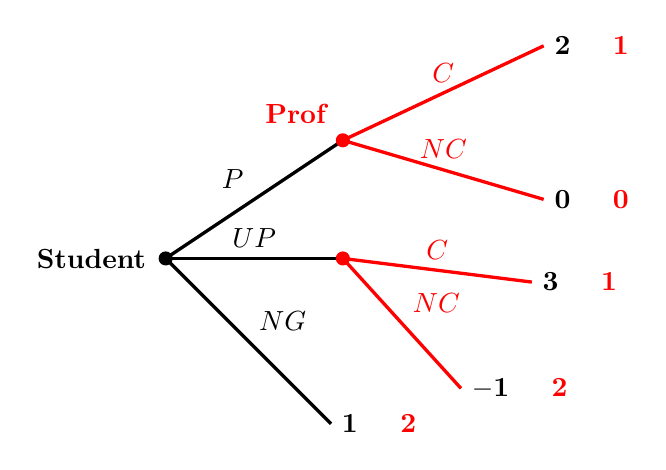
\begin{tikzpicture}[
    scale=1.5,
    font=\bfseries,
    dot/.style={circle, fill=#1, inner sep=1.8pt},
    dot/.default=black,
    line width=1.2pt
]

    % Coordinates
    \coordinate (root)   at (0, 0);
    \coordinate (qg_top) at (1.5, 1);
    \coordinate (qg_mid) at (1.5, 0);
    \coordinate (leaf_ng) at (1.4, -1.4);
    
    \coordinate (leaf1) at (3.2, 1.8);
    \coordinate (leaf2) at (3.2, 0.5);
    \coordinate (leaf3) at (3.1, -0.2);
    \coordinate (leaf4) at (2.5, -1.1);

    % Level 1 branches (You - Black)
    \draw[black] (root) -- (qg_top) node[midway, above left] {$P$};
    \draw[black] (root) -- (qg_mid) node[midway, above] {$UP$};
    \draw[black] (root) -- (leaf_ng) node[midway, above right] {$NG$};

    % Level 2 branches (QG - Red)
    \draw[red] (qg_top) -- (leaf1) node[midway, above] {$C$};
    \draw[red] (qg_top) -- (leaf2) node[midway, above] {$NC$};
    \draw[red] (qg_mid) -- (leaf3) node[midway, above] {$C$};
    \draw[red] (qg_mid) -- (leaf4) node[midway, above right] {$NC$};

    % Nodes & Labels
    \node[dot=black, label=left:Student] at (root) {};
    \node[dot=red, label={[red]above left:Prof}] at (qg_top) {};
    \node[dot=red] at (qg_mid) {};

    % Payoffs (You: black, QG: red)
    \node[right] at (leaf1) {2 \quad \textcolor{red}{1}};
    \node[right] at (leaf2) {0 \quad \textcolor{red}{0}};
    \node[right] at (leaf3) {3 \quad \textcolor{red}{1}};
    \node[right] at (leaf4) {$-$1 \quad \textcolor{red}{2}};
    \node[right] at (leaf_ng) {1 \quad \textcolor{red}{2}};

\end{tikzpicture}
\end{document}

    }
    \end{figure}
    \begin{itemize}
        \item By backward induction, we can find that in the unique SPE, the professor always complies if the student is prepared and never complies if the student is unprepared.
        \item The professor makes different moves depending on whether the student is prepared or not.
        \item However, what if he doesn't know if the student is prepared?
    \end{itemize}

    \item In a dynamic game with imperfect information:
    \begin{itemize}
        \item A player has some \textbf{information sets}, which contain histories that they cannot tell apart. For example:
        
        \begin{figure}[h]
        \centering
        \resizebox{0.3\textwidth}{!}{
        \documentclass[tikz,border=5mm]{standalone}
\usepackage{xcolor}

\definecolor{trafficgreen}{RGB}{34, 139, 34}
\definecolor{trafficyellow}{RGB}{204, 170, 0}
\definecolor{gameblue}{RGB}{0, 102, 204}

\begin{document}
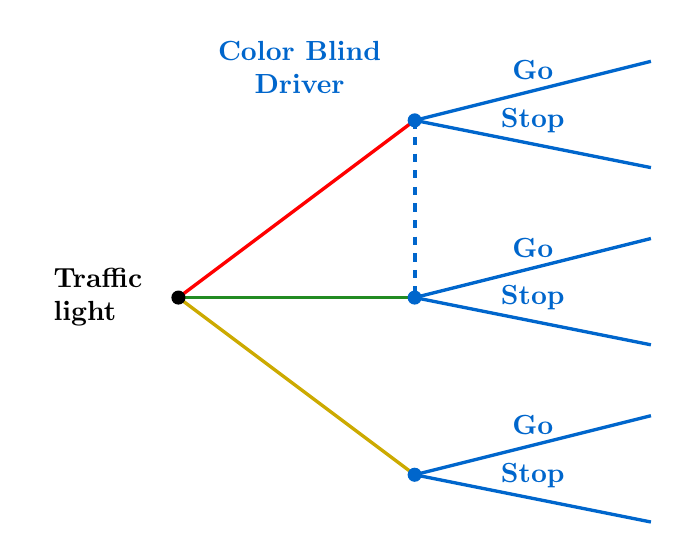
\begin{tikzpicture}[
    scale=1.5,
    font=\bfseries,
    dot/.style={circle, fill=#1, inner sep=1.8pt},
    dot/.default=black,
    line width=1.2pt
]

    % Coordinates
    \coordinate (root)       at (0, 0);
    \coordinate (driver_top) at (2, 1.5);
    \coordinate (driver_mid) at (2, 0);
    \coordinate (driver_bot) at (2, -1.5);
    
    \coordinate (l1_go)   at (4, 2.0);
    \coordinate (l1_stop) at (4, 1.1);
    
    \coordinate (l2_go)   at (4, 0.5);
    \coordinate (l2_stop) at (4, -0.4);
    
    \coordinate (l3_go)   at (4, -1.0);
    \coordinate (l3_stop) at (4, -1.9);

    % Level 1 branches (Traffic light signals)
    \draw[red] (root) -- (driver_top);
    \draw[trafficgreen] (root) -- (driver_mid);
    \draw[trafficyellow] (root) -- (driver_bot);

    % Information Set (Dashed Blue Line for Color Blind Driver)
    \draw[gameblue, dashed, line width=1.5pt] (driver_top) -- (driver_mid);

    % Level 2 branches (Color Blind Driver - Blue)
    \draw[gameblue] (driver_top) -- (l1_go)   node[midway, above] {Go};
    \draw[gameblue] (driver_top) -- (l1_stop) node[midway, above] {Stop};
    
    \draw[gameblue] (driver_mid) -- (l2_go)   node[midway, above] {Go};
    \draw[gameblue] (driver_mid) -- (l2_stop) node[midway, above] {Stop};
    
    \draw[gameblue] (driver_bot) -- (l3_go)   node[midway, above] {Go};
    \draw[gameblue] (driver_bot) -- (l3_stop) node[midway, above] {Stop};

    % Nodes & Labels
    \node[dot=black, align=left, label=left:\begin{tabular}{l}Traffic\\light\end{tabular}] at (root) {};
    \node[dot=gameblue, label={[gameblue]above left:\begin{tabular}{c}Color Blind\\Driver\end{tabular}}] at (driver_top) {};
    \node[dot=gameblue] at (driver_mid) {};
    \node[dot=gameblue] at (driver_bot) {};

\end{tikzpicture}
\end{document}

        }
        \end{figure}

        \item If the driver is normal, he has three information sets: \(\{red\}, \{green\}, \{yellow\}\). However, a color blind driver only has two: \(\{red, green\}, \{yellow\}\)
        \item A player can only play a strategy for each information set \(I\), i.e. what they see.
    \end{itemize}

    \item How do players make decisions under imperfect information?
    \begin{itemize}
        \item They have \textbf{belief} for what is going to be played in any information set.
    \end{itemize}

    \item Formally, a \textbf{belief system} \(\mu\) constitutes of beliefs \(\mu(x)\) for all \(x\) in any information set \(I\), where \(\sum_{x\in I}\mu(x) = 1\), which assigns conditional probabilities of being at history \(x\) given that information set \(I\) has been reached.

    \item \textbf{Example 5.1.1. Asking for Extra Credit with Imperfect Information.} Suppose the professor doesn't know if the student who comes is prepared or not. However, he believes that the student is prepared with probability \(\mu(P) = p\).
    
    \begin{figure}[h]
        \centering
        \resizebox{0.3\textwidth}{!}{
        \input{pupbelief}
        }
    \end{figure}
    
    Then, the professor should make their decision based on their expected utility:
    \[
    \begin{cases}
        U_P(C) = 1 \cdot p + 1 \cdot (1-p) = 1  \\
        U_P(NC) = 0 \cdot p + 2 \cdot (1-p) = 2-2p
    \end{cases}
    \]
    Therefore, complying is a best response if and only if \(1 \ge 2-2p \implies p \ge 0.5\).

    %\newpage
    Consider this strategy profile where \(p=1\):
    \begin{figure}[h]
        \centering
        \resizebox{0.3\textwidth}{!}{
        \input{pupbelief1}
        }
    \end{figure}
    \begin{itemize}
        \item \(p=1 \ge 0.5 \implies C\) is a best response according to the professor's belief.
        \item If the student somehow knows the professor's belief and thus what they will do, by backward induction they should not prepare
        \item However, the professor believes that the student is prepared, so the belief is \textbf{inconsistent}.
    \end{itemize}

    \item In a dynamic game with imperfect information, an equilibrium does not only require best response, but two conditions.
    \item \textbf{Definition 5.1.} A \textbf{perfect Bayesian equilibrium (PBE)} is a pair consisting of a strategy profile \(\sigma\) and a belief system \(\mu\), where:
    \begin{enumerate}
        \item \textbf{Sequential rationality}: For each player, their equilibrium strategy is a best response against other players' equilibrium strategies in every information set after which they move with respect to the beliefs given by \(\mu\).
        \item \textbf{Belief consistency}: For each player, their belief given by \(\mu\) is consistent with \(\sigma\) by conditional probability computed by Bayes' rule.
    \end{enumerate}

    \item In the previous example, (1) is satisfied but (2) is not. We use a mixed strategy example to show the other case.

    \begin{figure}[h]
        \centering
        \resizebox{0.3\textwidth}{!}{
        \documentclass[tikz,border=5mm]{standalone}
\usepackage{xcolor}
\usetikzlibrary{decorations.markings, arrows.meta}

\definecolor{gamegreen}{RGB}{58, 107, 34}

\begin{document}
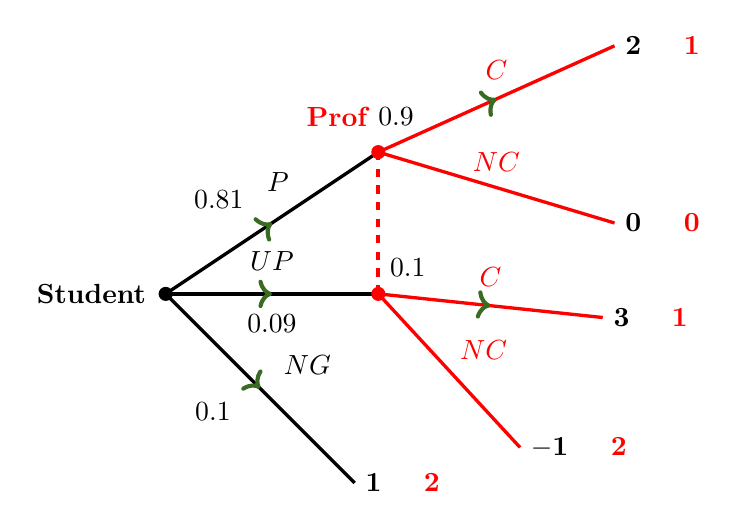
\begin{tikzpicture}[
    scale=1.5,
    font=\bfseries,
    dot/.style={circle, fill=#1, inner sep=1.8pt},
    dot/.default=black,
    line width=1.2pt,
    % Style to put a green arrow along the branch
    green arrow/.style={
        postaction={
            decorate,
            decoration={
                markings,
                mark=at position 0.5 with {
                    \arrow[gamegreen, line width=1.5pt]{>};
                }
            }
        }
    }
]

    % Coordinates
    \coordinate (root)    at (0, 0);
    \coordinate (qg_top)  at (1.8, 1.2);
    \coordinate (qg_mid)  at (1.8, 0);
    \coordinate (leaf_ng) at (1.6, -1.6);
    
    \coordinate (leaf1) at (3.8, 2.1);
    \coordinate (leaf2) at (3.8, 0.6);
    \coordinate (leaf3) at (3.7, -0.2);
    \coordinate (leaf4) at (3.0, -1.3);

    % Level 1 branches (You - Black)
    \draw[black, green arrow] (root) -- (qg_top);
    \node at (0.45, 0.8) {$0.81$};
    \node at (0.95, 0.95) {$P$};

    \draw[black, green arrow] (root) -- (qg_mid);
    \node at (0.9, 0.28) {$UP$};
    \node at (0.9, -0.25) {$0.09$};

    \draw[black, green arrow] (root) -- (leaf_ng);
    \node at (1.2, -0.6) {$NG$};
    \node at (0.4, -1.0) {$0.1$};

    % Information Set (Dashed Red Line)
    \draw[red, dashed, line width=1.5pt] (qg_top) -- (qg_mid);

    % Level 2 branches (QG - Red)
    \draw[red, green arrow] (qg_top) -- (leaf1) node[midway, above=3pt] {$C$};
    \draw[red] (qg_top) -- (leaf2) node[midway, above=2pt] {$NC$};
    
    \draw[red, green arrow] (qg_mid) -- (leaf3) node[midway, above=3pt] {$C$};
    \draw[red] (qg_mid) -- (leaf4) node[midway, above right] {$NC$};

    % Nodes & Labels
    \node[dot=black, label=left:Student] at (root) {};
    \node[dot=red] at (qg_top) {};
    \node[dot=red] at (qg_mid) {};

    % Un-overlapped labels for QG and beliefs (0.9, 0.1)
    \node[red]   at (1.45, 1.5) {Prof};
    \node[black] at (1.95, 1.5) {$0.9$};
    \node[black] at (2.05, 0.22) {$0.1$};

    % Payoffs (You: black, QG: red)
    \node[right] at (leaf1) {2 \quad \textcolor{red}{1}};
    \node[right] at (leaf2) {0 \quad \textcolor{red}{0}};
    \node[right] at (leaf3) {3 \quad \textcolor{red}{1}};
    \node[right] at (leaf4) {$-$1 \quad \textcolor{red}{2}};
    \node[right] at (leaf_ng) {1 \quad \textcolor{red}{2}};

\end{tikzpicture}
\end{document}

        }
    \end{figure}
    \begin{itemize}
        \item Is this belief consistent?
        \item Suppose the professor sees a student comes, then:
        \[
        \mathbb{P}(P \mid \{P, UP\}) = \frac{\mathbb{P}(P)}{\mathbb{P}(\{P, UP\})} = \frac{0.81}{0.81+0.09} = 0.9
        \]
        which is consistent with the belief \(p=0.9\).
        \item However, if the professor must comply, the student's best response is to never prepare, instead of playing this mixed strategy.
    \end{itemize}

    \item In practice, one way to find a PBE can be seen as a more complicated backward induction:
    \begin{enumerate}
        \item For the last player(s), find what are the best responses under all conditions of their belief.
        \item For every possible actions, find the best responses the previous player can take.
        \item Check if this action is consistent with the belief.
    \end{enumerate}

    \item In the previous example, there are two possibilities in step (1):
    \item If \(p \ge 0.5\) and the professor complies:
    \begin{itemize}
        \item The student should not prepare by backward induction.
        \item Then, the actual probability of the student preparing is 0, as opposed to the belief \(p \ge 0.5\).
        \item Belief consistency is violated: No valid PBE under this belief.
    \end{itemize}
    \item If \(p \le 0.5\) and the professor does not comply:
    \begin{itemize}
        \item By backward induction, the student must not go to the office.
        \item Is belief consistent?
        \item Checking by Bayes' rule:
        \[
        \mathbb{P}(P \mid \{P, UP\}) = \frac{\mathbb{P}(P)}{\mathbb{P}(\{P, UP\})} = \frac{0}{0}?
        \]
        \item What happened here?
        \item There are \textbf{off-equilibrium paths}. In fact, if nothing in an information set is played, one is allowed to have any belief.
        \item PBE: Student never goes, Professor believes in any \(p \le 0.5\) and (hypothetically) never complies.
    \end{itemize}
    
\end{itemize}

\subsection{Incomplete Information}

\begin{itemize}
    \item What's the difference between \textbf{imperfect} and \textbf{incomplete} information?
    \begin{itemize}
        \item Under imperfect information, you don't know what your opponent has played. Under incomplete information, you simply don't know who your opponent is; or to be precise, the \textbf{type} of your opponent.
    \end{itemize}
    %\newpage
    \item \textbf{Example 5.2. Asking for Extra Credit with Incomplete Information.} Suppose there are two types of students, Eagle and Dove. The student is an Eagle with probability \(q\).
    \begin{figure}[h]
        \centering
        \resizebox{0.4\textwidth}{!}{
        \documentclass[tikz,border=5mm]{standalone}
\usepackage{xcolor}

\definecolor{gameblue}{RGB}{0, 102, 204}

\begin{document}
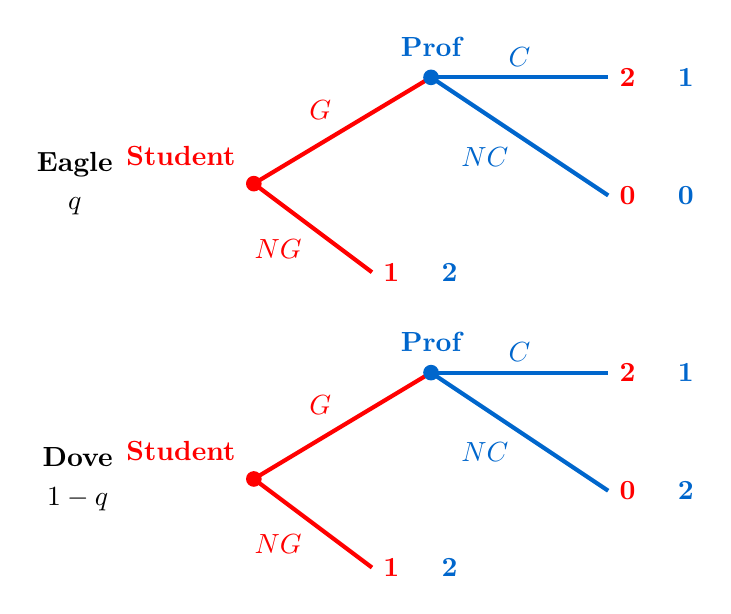
\begin{tikzpicture}[
    scale=1.5,
    font=\bfseries,
    dot/.style={circle, fill=#1, inner sep=2pt},
    dot/.default=black,
    line width=1.5pt
]

    % ==========================================
    % TOP TREE (Eagle / q)
    % ==========================================
    \coordinate (t_root)    at (0, 0);
    \coordinate (t_qg)      at (1.5, 0.9);
    \coordinate (t_ng)      at (1.0, -0.75);
    \coordinate (t_leaf_c)  at (3.0, 0.9);
    \coordinate (t_leaf_nc) at (3.0, -0.1);

    % Level 1 branches (Student - Red)
    \draw[red] (t_root) -- (t_qg) node[midway, above left] {$G$};
    \draw[red] (t_root) -- (t_ng) node[midway, below left] {$NG$};

    % Level 2 branches (Prof - Blue)
    \draw[gameblue] (t_qg) -- (t_leaf_c)  node[midway, above] {$C$};
    \draw[gameblue] (t_qg) -- (t_leaf_nc) node[midway, below left] {$NC$};

    % Nodes & Labels (Student placed 'above left', Eagle shifted further left)
    \node[dot=red, label={[red, anchor=south east]above left:Student}] at (t_root) {};
    \node[dot=gameblue, label={[gameblue]above:Prof}] at (t_qg) {};
    \node[align=center, anchor=east] at (-1.1, 0) {Eagle\\[2pt]$q$};

    % Payoffs (Red \quad Blue)
    \node[right] at (t_ng)      {\textcolor{red}{1} \quad \textcolor{gameblue}{2}};
    \node[right] at (t_leaf_c)  {\textcolor{red}{2} \quad \textcolor{gameblue}{1}};
    \node[right] at (t_leaf_nc) {\textcolor{red}{0} \quad \textcolor{gameblue}{0}};


    % ==========================================
    % BOTTOM TREE (Dove / 1-q)
    % ==========================================
    \coordinate (b_root)    at (0, -2.5);
    \coordinate (b_qg)      at (1.5, -1.6);
    \coordinate (b_ng)      at (1.0, -3.25);
    \coordinate (b_leaf_c)  at (3.0, -1.6);
    \coordinate (b_leaf_nc) at (3.0, -2.6);

    % Level 1 branches (Student - Red)
    \draw[red] (b_root) -- (b_qg) node[midway, above left] {$G$};
    \draw[red] (b_root) -- (b_ng) node[midway, below left] {$NG$};

    % Level 2 branches (Prof - Blue)
    \draw[gameblue] (b_qg) -- (b_leaf_c)  node[midway, above] {$C$};
    \draw[gameblue] (b_qg) -- (b_leaf_nc) node[midway, below left] {$NC$};

    % Nodes & Labels (Student placed 'above left', Dove shifted further left)
    \node[dot=red, label={[red, anchor=south east]above left:Student}] at (b_root) {};
    \node[dot=gameblue, label={[gameblue]above:Prof}] at (b_qg) {};
    \node[align=center, anchor=east] at (-1.1, -2.5) {Dove\\[2pt]$1-q$};

    % Payoffs (Red \quad Blue)
    \node[right] at (b_ng)      {\textcolor{red}{1} \quad \textcolor{gameblue}{2}};
    \node[right] at (b_leaf_c)  {\textcolor{red}{2} \quad \textcolor{gameblue}{1}};
    \node[right] at (b_leaf_nc) {\textcolor{red}{0} \quad \textcolor{gameblue}{2}};

\end{tikzpicture}
\end{document}

        }
    \end{figure}
    \item In fact, such game can be transformed into a game with imperfect information by something called \textbf{Harsanyi transformation}.
    \item We introduce an additional player called \textbf{Nature}.
    \begin{itemize}
        \item Nature plays a fixed mixed strategy that determines players' types, and this move is only observed by that player.
        \item Nature is non-strategic: It doesn't optimize, but belief still needs to be consistent.
    \end{itemize}
    %\newpage
    \begin{figure}[h]
        \centering
        \resizebox{0.4\textwidth}{!}{
        \documentclass[tikz,border=5mm]{standalone}
\usepackage{xcolor}

\definecolor{gameblue}{RGB}{0, 102, 204}
\definecolor{gamered}{RGB}{204, 51, 34}

\begin{document}
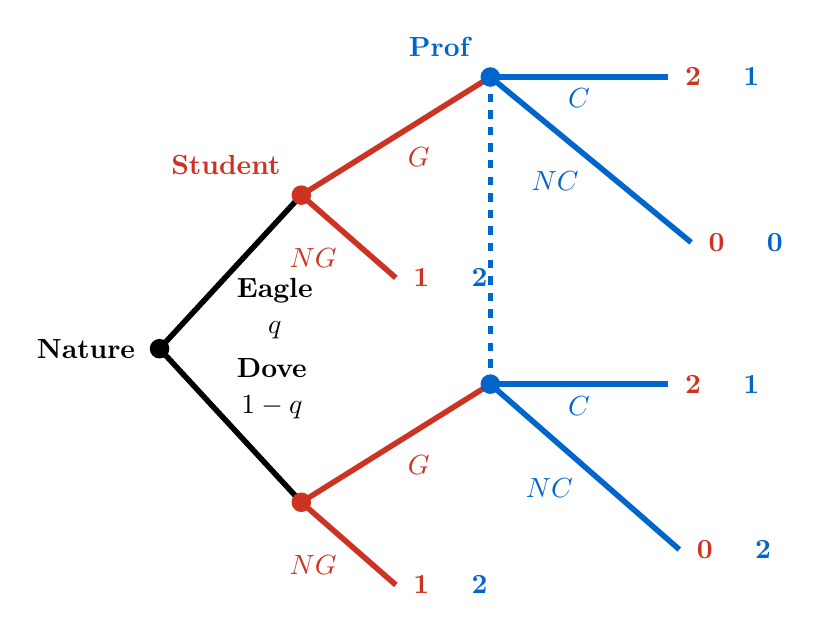
\begin{tikzpicture}[
    scale=1.5,
    font=\bfseries,
    dot/.style={circle, fill=#1, inner sep=2.5pt},
    dot/.default=black,
    line width=2pt
]

    % --- Coordinates ---
    % Nature Root
    \coordinate (nature)   at (0, 0);

    % Top Subtree (Eagle)
    \coordinate (t_you)     at (1.2, 1.3);
    \coordinate (t_qg)      at (2.8, 2.3);
    \coordinate (t_ng)      at (2.0, 0.6);
    \coordinate (t_leaf_c)  at (4.3, 2.3);
    \coordinate (t_leaf_nc) at (4.5, 0.9);

    % Bottom Subtree (Dove)
    \coordinate (b_you)     at (1.2, -1.3);
    \coordinate (b_qg)      at (2.8, -0.3);
    \coordinate (b_ng)      at (2.0, -2.0);
    \coordinate (b_leaf_c)  at (4.3, -0.3);
    \coordinate (b_leaf_nc) at (4.4, -1.7);

    % --- Level 0: Nature Branches ---
    \draw[black] (nature) -- (t_you) node[midway, below right, align=center, xshift=-2pt, yshift=2pt] {Eagle\\[1pt]$q$};
    \draw[black] (nature) -- (b_you) node[midway, above right, align=center, xshift=-2pt, yshift=-2pt] {Dove\\[1pt]$1-q$};

    % --- Level 1: "You" Branches (Red) ---
    \draw[gamered] (t_you) -- (t_qg) node[midway, below right] {$G$};
    \draw[gamered] (t_you) -- (t_ng) node[midway, below left] {$NG$};

    \draw[gamered] (b_you) -- (b_qg) node[midway, below right] {$G$};
    \draw[gamered] (b_you) -- (b_ng) node[midway, below left] {$NG$};

    % --- Information Set (Dashed Line connecting QG nodes) ---
    \draw[gameblue, dashed, line width=2pt] (t_qg) -- (b_qg);

    % --- Level 2: "QG" Branches (Blue) ---
    \draw[gameblue] (t_qg) -- (t_leaf_c)  node[midway, below] {$C$};
    \draw[gameblue] (t_qg) -- (t_leaf_nc) node[midway, below left] {$NC$};

    \draw[gameblue] (b_qg) -- (b_leaf_c)  node[midway, below] {$C$};
    \draw[gameblue] (b_qg) -- (b_leaf_nc) node[midway, below left] {$NC$};

    % --- Nodes & Decision Labels ---
    \node[dot=black, label={[black]left:Nature}] at (nature) {};

    \node[dot=gamered, label={[gamered]above left:Student}] at (t_you) {};
    \node[dot=gamered] at (b_you) {};

    \node[dot=gameblue, label={[gameblue]above left:Prof}] at (t_qg) {};
    \node[dot=gameblue] at (b_qg) {};

    % --- Payoffs: Red (You) \quad Blue (QG) ---
    % Top tree payoffs
    \node[right=2pt] at (t_ng)      {\textcolor{gamered}{1} \quad \textcolor{gameblue}{2}};
    \node[right=2pt] at (t_leaf_c)  {\textcolor{gamered}{2} \quad \textcolor{gameblue}{1}};
    \node[right=2pt] at (t_leaf_nc) {\textcolor{gamered}{0} \quad \textcolor{gameblue}{0}};

    % Bottom tree payoffs
    \node[right=2pt] at (b_ng)      {\textcolor{gamered}{1} \quad \textcolor{gameblue}{2}};
    \node[right=2pt] at (b_leaf_c)  {\textcolor{gamered}{2} \quad \textcolor{gameblue}{1}};
    \node[right=2pt] at (b_leaf_nc) {\textcolor{gamered}{0} \quad \textcolor{gameblue}{2}};

\end{tikzpicture}
\end{document}

        }
    \end{figure}

    \item Instead of the method in the last section, another way to find PBEs is to analyze different candidate strategy profiles.
    \item We first classify two types of strategy profiles:
    \begin{itemize}
        \item \textbf{Separating}: Different types play different strategies.
        \item \textbf{Pooling}: Different types play the same strategy.
    \end{itemize}

    \item In this game, there are four candidates:
    \begin{enumerate}
        \item Separating: Eagle goes, Dove does not
        \begin{itemize}
            \item For belief to be consistent, the professor must believe whoever comes is an Eagle. Best response is to always comply.
            \item However, Dove can then choose to go instead to ``pretend" to be an Eagle. As not going is not a best response for Dove, this is not a PBE.
        \end{itemize}
        \item Separating: Dove goes, Eagle does not
        \begin{itemize}
            \item For belief to be consistent, the professor must believe whoever comes is an Dove. Best response is to never comply.
            \item Knowing this, Dove should never go. As going is not a best response for Dove, this is not a PBE.
        \end{itemize}
        \item Pooling: Both go
        \begin{itemize}
            \item For belief to be consistent, the professor must believe in the ``true" probability: the student who comes is Eagle with probability \(q\) and Dove with probability \(1-q\).
            \item Then, the expected utility is:
            \[
            \begin{cases}
                U_P(C) = 1 \cdot q + 1 \cdot (1-q) = 1  \\
                U_P(NC) = 0 \cdot q + 2 \cdot (1-q) = 2-2q
            \end{cases}
            \]
            \item If \(q \le 0.5\), not complying is a best response. However, if the professor does not comply, going is not a best response for both. This is not a PBE.
            \item If \(q \ge 0.5\), complying is a best response. Going is then also a best response for both types. This is a PBE.
        \end{itemize}
        \item Pooling: Both don't go
        \begin{itemize}
            \item Since the information set \(\{(Eagle, G),(Dove,G)\}\) is not reached, the professor is free to have any belief. Let \(p\) be the belief that the student is Eagle.
            \item If \(p \ge 0.5\), complying is a best response. However, if the professor always complies, not going is not a best response for both. This is not a PBE.
            \item If \(p \le 0.5\), not complying is a best response. Not going is then also a best response for both types. This is a PBE.
        \end{itemize}
    \end{enumerate}

    \item \textbf{Example 5.3. Akerlof's Lemon Market (Screening Game).} A seller is selling a used car with value \(v \in [0,1]\). The car is worth \(v\) to a buyer, but only \(\alpha v\) to the seller, where \(\alpha \in [0,1]\). The buyer first proposes a price \(p\) to the seller, and the seller decides to accept or reject the deal. If the deal is accepted, the seller gets \(p-\alpha v\) and the buyer gets \(v-p\); otherwise, both walk away with 0.

    \begin{itemize}
        \item In a basic demand-and-supply model with complete information, the trade will take place at any \(p \in [\alpha v, v]\), since both can be better off.
        \item However, with incomplete information, the buyer doesn't know \(v\), but only the probability distribution: \(v \sim \text{Uniform}(0,1)\).
        \item Will there be a deal?
        \item Suppose the buyer proposes any arbitrary \(p \in [0,1]\).
        \item Note that the seller will accept if \(p-\alpha v > 0\), and reject if \(p-\alpha v < 0\).
        \item Clearly, the only possible sellers who will accept are those with \(v \in [0,\frac{p}{\alpha}]\).
        \item Going back to the buyer, did they make a reasonable offer?
        \item We calculate the expected utility of proposing \(p\):
        \[
        U_B(p) = \mathbb{P}(v \in [0,\frac{p}{\alpha}]) \cdot \mathbb{E}(v-p \mid v \in [0,\frac{p}{\alpha}]) = \frac{p}{\alpha} \cdot (\frac{p}{2\alpha} - p) = \frac{p^2}{2\alpha^2} \cdot (1-2\alpha)
        \]
        \item If \(\alpha \ge 0.5\), proposing any \(p>0\) will in fact produce negative payoff!
        \item \textbf{Winner's curse}: The seller accepting the deal implies that the car actually isn't worth as much.
        \item In this case, the buyer wants the seller to reject the offer all the time. The PBE is offering \(p=0\) and getting rejected.
        \item If \(\alpha \le 0.5\), the optimal offer is simply a boundary solution: \(p = \alpha\), where every type of seller will accept the offer.
    \end{itemize}

    \item \textbf{Example 5.4. Job Market Signaling.} A player, Alice, is born Smart or Average. She first decides to go to college or not. Then, a firm decides to offer Alice a High or a Low job. The firm only sees whether Alice has gone to college, but not whether she is Smart.

    Alice's payoff is coming from the value of the job minus the cost of going to college, where the only difference is that going to college is more (mentally) costly for Average Alice.

    \begin{center}
    \renewcommand{\arraystretch}{1.5}
    \begin{tabular}{lll}
    & High job: $+10$ & Low job: $+5$ \\
    Going to college:     & Smart: $-2$ & Average: $-10$ \\
    Not going to college: & Smart: $-0$ & Average: $-0$  \\
    \end{tabular}
    \end{center}

    The firm wants to match the right person to the right job.

    \begin{center}
    \renewcommand{\arraystretch}{1.5}
    \begin{tabular}{lll}
    Smart \& High: $+10$ & Average \& Low: $+5$ & Otherwise: $0$ \\
    \end{tabular}
    \end{center}

    \newpage
    Using a game tree to represent:
    \begin{figure}[h]
        \centering
        \resizebox{0.4\textwidth}{!}{
        \documentclass[tikz,border=5mm]{standalone}
\usepackage{xcolor}

\definecolor{gameblue}{RGB}{0, 102, 204}

\begin{document}
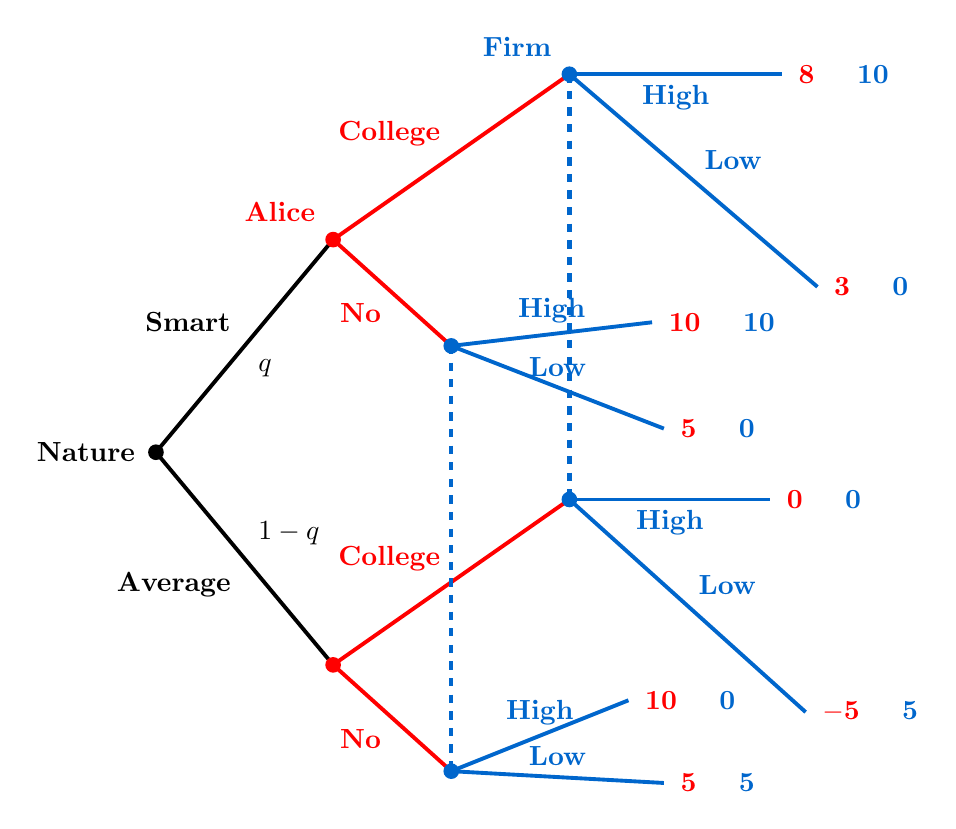
\begin{tikzpicture}[
    scale=1.5,
    font=\bfseries,
    dot/.style={circle, fill=#1, inner sep=2pt},
    dot/.default=black,
    line width=1.4pt
]

    % ==========================================
    % COORDINATES
    % ==========================================
    % Root (Nature)
    \coordinate (root) at (0, 0);

    % Alice's Nodes
    \coordinate (alice_top) at (1.5, 1.8);
    \coordinate (alice_bot) at (1.5, -1.8);

    % Firm's Nodes (College: x = 3.5, No: x = 2.5)
    \coordinate (firm_tc) at (3.5, 3.2);  % Top College
    \coordinate (firm_tn) at (2.5, 0.9);  % Top No
    \coordinate (firm_bc) at (3.5, -0.4); % Bottom College
    \coordinate (firm_bn) at (2.5, -2.7); % Bottom No

    % Payoff Endpoints - Top College
    \coordinate (l_tc_high) at (5.3, 3.2);
    \coordinate (l_tc_low)  at (5.6, 1.4);

    % Payoff Endpoints - Top No
    \coordinate (l_tn_high) at (4.2, 1.1);
    \coordinate (l_tn_low)  at (4.3, 0.2);

    % Payoff Endpoints - Bottom College
    \coordinate (l_bc_high) at (5.2, -0.4);
    \coordinate (l_bc_low)  at (5.5, -2.2);

    % Payoff Endpoints - Bottom No
    \coordinate (l_bn_high) at (4.0, -2.1);
    \coordinate (l_bn_low)  at (4.3, -2.8);


    % ==========================================
    % LEVEL 1: NATURE (Black)
    % ==========================================
    \draw[black] (root) -- (alice_top) 
        node[midway, above left=1pt] {Smart}
        node[midway, below right=1pt] {$q$};
        
    \draw[black] (root) -- (alice_bot) 
        node[midway, below left=1pt] {Average}
        node[midway, above right=1pt] {$1-q$};


    % ==========================================
    % LEVEL 2: ALICE (Red)
    % ==========================================
    % Top Alice
    \draw[red] (alice_top) -- (firm_tc) node[midway, above left] {College};
    \draw[red] (alice_top) -- (firm_tn) node[midway, below left] {No};

    % Bottom Alice
    \draw[red] (alice_bot) -- (firm_bc) node[midway, above left] {College};
    \draw[red] (alice_bot) -- (firm_bn) node[midway, below left] {No};


    % ==========================================
    % INFORMATION SETS (Firm - Blue Dashed)
    % ==========================================
    \draw[gameblue, dashed, line width=1.6pt] (firm_tc) -- (firm_bc);
    \draw[gameblue, dashed, line width=1.6pt] (firm_tn) -- (firm_bn);


    % ==========================================
    % LEVEL 3: FIRM (Blue)
    % ==========================================
    % Top College
    \draw[gameblue] (firm_tc) -- (l_tc_high) node[midway, below] {High};
    \draw[gameblue] (firm_tc) -- (l_tc_low)  node[midway, above right] {Low};

    % Top No
    \draw[gameblue] (firm_tn) -- (l_tn_high) node[midway, above] {High};
    \draw[gameblue] (firm_tn) -- (l_tn_low)  node[midway, above] {Low};

    % Bottom College
    \draw[gameblue] (firm_bc) -- (l_bc_high) node[midway, below] {High};
    \draw[gameblue] (firm_bc) -- (l_bc_low)  node[midway, above right] {Low};

    % Bottom No
    \draw[gameblue] (firm_bn) -- (l_bn_high) node[midway, above] {High};
    \draw[gameblue] (firm_bn) -- (l_bn_low)  node[midway, above] {Low};


    % ==========================================
    % NODES & PLAYER LABELS
    % ==========================================
    \node[dot=black, label=left:Nature] at (root) {};
    
    \node[dot=red, label={[red]above left:Alice}] at (alice_top) {};
    \node[dot=red] at (alice_bot) {};
    
    \node[dot=gameblue, label={[gameblue]above left:Firm}] at (firm_tc) {};
    \node[dot=gameblue] at (firm_tn) {};
    \node[dot=gameblue] at (firm_bc) {};
    \node[dot=gameblue] at (firm_bn) {};


    % ==========================================
    % PAYOFFS (Alice: Red, Firm: Blue)
    % ==========================================
    % Top College
    \node[right=2pt] at (l_tc_high) {\textcolor{red}{8} \quad \textcolor{gameblue}{10}};
    \node[right=2pt] at (l_tc_low)  {\textcolor{red}{3} \quad \textcolor{gameblue}{0}};

    % Top No
    \node[right=2pt] at (l_tn_high) {\textcolor{red}{10} \quad \textcolor{gameblue}{10}};
    \node[right=2pt] at (l_tn_low)  {\textcolor{red}{5} \quad \textcolor{gameblue}{0}};

    % Bottom College
    \node[right=2pt] at (l_bc_high) {\textcolor{red}{0} \quad \textcolor{gameblue}{0}};
    \node[right=2pt] at (l_bc_low)  {\textcolor{red}{$-$5} \quad \textcolor{gameblue}{5}};

    % Bottom No
    \node[right=2pt] at (l_bn_high) {\textcolor{red}{10} \quad \textcolor{gameblue}{0}};
    \node[right=2pt] at (l_bn_low)  {\textcolor{red}{5} \quad \textcolor{gameblue}{5}};

\end{tikzpicture}
\end{document}

        }
    \end{figure}
    \begin{itemize}
        \item To Alice, going to college is strictly worse off. To the firm, what actually matters is the type of Alice but not her degree. Would Alice go to college at all?
        \item Notice that Average Alice must not attend college in any PBE, as the best she can get from going to college (College \& High job) is still not as good as the worst she can get from not going (No College \& Low job).
        \item So, we only need to consider Smart Alice.
    \end{itemize}
    \begin{enumerate}
        \item Separating: Smart Alice goes to college, Average Alice does not
        \begin{itemize}
            \item For belief to be consistent, the firm must believe whoever went to college is Smart, and whoever did not is Average.
            \item Best response: Offer High job to who went to college, and Low job to who didn't.
            \item This is a PBE.
        \end{itemize}
        \item Pooling: Both don't go to college
        \begin{itemize}
            \item Because there are two information sets with more than one histories, \(\{(Smart, College), \)
            
            \((Average, College)\}\) and \(\{(Smart, No College), (Average, No College)\}\), the firm should have two sets of beliefs.
            \item For belief to be consistent, the firm must believe in the ``true" probability if they see an Alice with no college degree: Alice is Smart with probability \(q\) and Average with probability \(1-q\).
            \item On the other hand, they can have any \textbf{off-equilibrium belief}, say \(p\) for Smart and \(1-p\) for Average, along the ``college" path and then take any hypothetical best response.
            \item When Alice does not go to college, the expected utility for the firm is:
            \[
            \begin{cases}
                U_F(H) &= 10q + 0(1-q) = 10q \\
                U_F(L) &= 0q + 5(1-q) = 5-5q
            \end{cases}
            \]
            Thus, the firm will offer High job if \(q \ge \frac{1}{3}\), and Low job if \(q \le \frac{1}{3}\).
        \end{itemize}
        \begin{enumerate}
            \item If \(q \ge \frac{1}{3}\) and the firm offers High job: Both types of Alice get the absolutely highest payoff (+10). This is a PBE.
            \item If \(q \le \frac{1}{3}\) and the firm offers Low job: 
        \end{enumerate}
        \begin{itemize}
            \item Can Smart Alice deviate to attend college?
            \item It depends on the firm's belief for a college-attending Alice.
            \item Note that because going to college has no value added at all, the firm's expected utility is almost identical:
            \[
            \begin{cases}
                U_F(H) &= 10p + 0(1-p) = 10p \\
                U_F(L) &= 0p + 5(1-p) = 5-5p
            \end{cases}
            \]
            \item The firm then hypothetically offers High job if \(p \ge \frac{1}{3}\), and Low job if \(p \le \frac{1}{3}\).
            \item Thus, if \(p \ge \frac{1}{3}\) and the firm will offer High job in this case, Smart Alice has incentive to go to college, which is not a PBE.
            \item A pooling PBE: \(q \le \frac{1}{3}\), \(p \le \frac{1}{3}\), Alice doesn't go to college all the time, the firm offers Low job all the time.
        \end{itemize}
    \end{enumerate}

    \begin{itemize}
        \item While we have confirmed that a polling PBE exists, does this make sense?
        \item We know that Average Alice must not go to college in any PBE. However, the pooling equilibrium requires that \(p \le \frac{1}{3}\), that is, the firm thinks that an Alice who went to college is unlikely to be Smart!
        \item Thus, we want to kick out some equilibria that are unreasonable, i.e. \textbf{equilibrium refinement}.
        \item \textbf{Intuitive criterion}: If an unexpected deviation occurs (e.g. Alice going to college in pooling equilibrium), the receiver (e.g. the firm) must assign zero probability to any sender type that could never benefit from that deviation under any plausible response (e.g. Average Alice).
        \item In this case, we must assign \(p=1\), which eliminates this polling equilibrium.
    \end{itemize}
    \item Some takeaways:
    \begin{enumerate}
        \item If a signaling mechanism (e.g. exam, job interview) is too weak to differentiate between strong and weak candidates (i.e. it is not too costly for weak candidates), it is possible that it fails to reach a separating equilibrium.
        \item If a separating equilibrium is available, Alice is willing to make herself slightly worse off for the sake of signaling. This is known in evolutionary biology as the \textbf{handicap principle}.
    \end{enumerate}

    \item \textbf{Example 5.5. Bayesian Persuasion.} The Governor calls the President and claims that there's an epidemic in his province, asking for a relief fund.

    The President decides whether to approve (\(Y\)) or reject (\(N\)) the request. He doesn't know if there is actually an epidemic, but a probability \(q<0.5\) of an epidemic. In contrast, the Governor knows the truth (state): whether there is an epidemic (\(y\)) or not (\(n\)).

    The Governor only wants the fund regardless of the truth: 
    \[u_G(Y) = 1 \text{ and } u_G(N) = 0\]
    The President wants it to match: 
    \[u_P(y,Y) = u_P(n,N) = 1 \text{ and } u_P(y,N) = u_P(n,Y) = 0\]
    Given a consistent belief, it follows that the expected utility for both are equivalent to the probabilities: 
    \[U_G = \mathbb{P}(Y), U_P(Y) = \mathbb{P}(y), U_P(N) = \mathbb{P}(n)\]

    \begin{itemize}
        \item If the state is more likely to be \(n\) (\(\mathbb{P}(y) = q<0.5\)), it is easy to verify that the President's best response is to always reject (\(N\)).
        \item The Governor always receives 0 and he cannot change the President's mind: a \textbf{cheap talk}.
        \item Potential solution: Invite a neutral inspector (e.g. WHO) to inspect, who always reports the truth to the president.
        \item Denote the reported state by \(\hat{y}\) or \(\hat{n}\). Since WHO always reports the truth, the President's best response is \(Y\) if \(\hat{y}\), and \(N\) if \(\hat{n}\).
        \item Then,
        \[
        U_G = q \cdot 1 + (1-q) \cdot 0 = q
        \]
        \item What if the Governor can hire an inspector who is not perfect or is not so honest?
        \item Suppose the Governor hires an inspector with ability \((\alpha, \beta)\), where \(\alpha\) is the probability of reporting \(\hat{y}\) if there is an epidemic, and \(\beta\) is the probability of reporting \(\hat{y}\) if there is not, and furthermore assume \(\alpha \ge \beta\).

        \newpage
        \begin{figure}[h]
        \centering
        \resizebox{0.4\textwidth}{!}{
        \documentclass[tikz,border=5mm]{standalone}
\usepackage{xcolor}

\definecolor{gameblue}{RGB}{0, 102, 204}
\definecolor{gamegreen}{RGB}{76, 175, 53}

\begin{document}
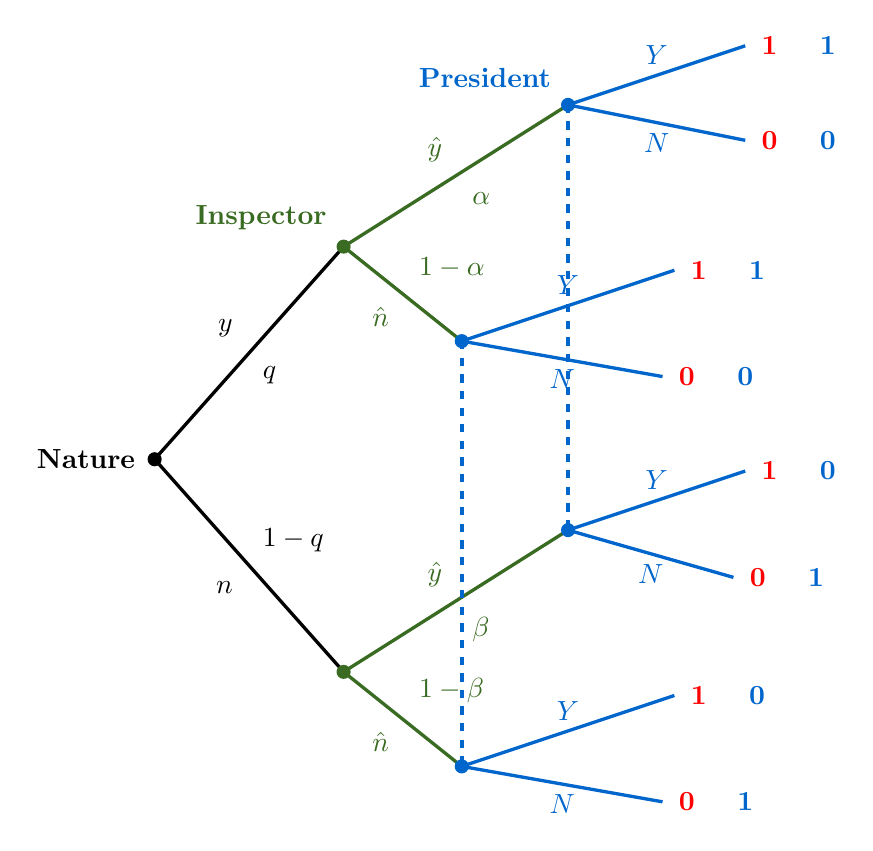
\begin{tikzpicture}[
    scale=1.5,
    font=\bfseries,
    dot/.style={circle, fill=#1, inner sep=1.8pt},
    dot/.default=black,
    line width=1.2pt
]

    % ==========================================
    % COORDINATES
    % ==========================================
    % Root (Nature)
    \coordinate (root) at (0, 0);

    % Inspector Nodes
    \coordinate (insp_top) at (1.6, 1.8);
    \coordinate (insp_bot) at (1.6, -1.8);

    % President Nodes
    \coordinate (pres_ty) at (3.5, 3.0);  % Top y-hat
    \coordinate (pres_tn) at (2.6, 1.0);  % Top n-hat
    \coordinate (pres_by) at (3.5, -0.6); % Bottom y-hat
    \coordinate (pres_bn) at (2.6, -2.6); % Bottom n-hat

    % Payoff Leaf Coordinates
    \coordinate (l_ty_Y) at (5.0, 3.5);
    \coordinate (l_ty_N) at (5.0, 2.7);

    \coordinate (l_tn_Y) at (4.4, 1.6);
    \coordinate (l_tn_N) at (4.3, 0.7);

    \coordinate (l_by_Y) at (5.0, -0.1);
    \coordinate (l_by_N) at (4.9, -1.0);

    \coordinate (l_bn_Y) at (4.4, -2.0);
    \coordinate (l_bn_N) at (4.3, -2.9);


    % ==========================================
    % LEVEL 1: NATURE (Black)
    % ==========================================
    \draw[black] (root) -- (insp_top) 
        node[midway, above left=2pt] {$y$}
        node[midway, below right=1pt] {$q$};
        
    \draw[black] (root) -- (insp_bot) 
        node[midway, below left=2pt] {$n$}
        node[midway, above right=1pt] {$1-q$};


    % ==========================================
    % LEVEL 2: INSPECTOR (Green)
    % ==========================================
    % Top Inspector branches
    \draw[gamegreen] (insp_top) -- (pres_ty) 
        node[midway, above left=1pt] {$\hat{y}$}
        node[midway, below right=2pt] {$\alpha$};
    \draw[gamegreen] (insp_top) -- (pres_tn) 
        node[midway, below left=1pt] {$\hat{n}$}
        node[midway, above right=2pt] {$1-\alpha$};

    % Bottom Inspector branches
    \draw[gamegreen] (insp_bot) -- (pres_by) 
        node[midway, above left=1pt] {$\hat{y}$}
        node[midway, below right=2pt] {$\beta$};
    \draw[gamegreen] (insp_bot) -- (pres_bn) 
        node[midway, below left=1pt] {$\hat{n}$}
        node[midway, above right=2pt] {$1-\beta$};


    % ==========================================
    % INFORMATION SETS (President - Blue Dashed)
    % ==========================================
    \draw[gameblue, dashed, line width=1.5pt] (pres_ty) -- (pres_by);
    \draw[gameblue, dashed, line width=1.5pt] (pres_tn) -- (pres_bn);


    % ==========================================
    % LEVEL 3: PRESIDENT (Blue)
    % ==========================================
    % Top y-hat branches
    \draw[gameblue] (pres_ty) -- (l_ty_Y) node[midway, above] {$Y$};
    \draw[gameblue] (pres_ty) -- (l_ty_N) node[midway, below] {$N$};

    % Top n-hat branches
    \draw[gameblue] (pres_tn) -- (l_tn_Y) node[midway, above] {$Y$};
    \draw[gameblue] (pres_tn) -- (l_tn_N) node[midway, below] {$N$};

    % Bottom y-hat branches
    \draw[gameblue] (pres_by) -- (l_by_Y) node[midway, above] {$Y$};
    \draw[gameblue] (pres_by) -- (l_by_N) node[midway, below] {$N$};

    % Bottom n-hat branches
    \draw[gameblue] (pres_bn) -- (l_bn_Y) node[midway, above] {$Y$};
    \draw[gameblue] (pres_bn) -- (l_bn_N) node[midway, below] {$N$};


    % ==========================================
    % NODES & PLAYER LABELS (Repositioned to avoid overlaps)
    % ==========================================
    \node[dot=black, label=left:Nature] at (root) {};
    
    \node[dot=gamegreen, label={[gamegreen]above left=2pt:Inspector}] at (insp_top) {};
    \node[dot=gamegreen] at (insp_bot) {};
    
    \node[dot=gameblue, label={[gameblue]above left=2pt:President}] at (pres_ty) {};
    \node[dot=gameblue] at (pres_tn) {};
    \node[dot=gameblue] at (pres_by) {};
    \node[dot=gameblue] at (pres_bn) {};


    % ==========================================
    % PAYOFFS (Inspector: Red, President: Blue)
    % ==========================================
    % From Top y-hat
    \node[right=2pt] at (l_ty_Y) {\textcolor{red}{1} \quad \textcolor{gameblue}{1}};
    \node[right=2pt] at (l_ty_N) {\textcolor{red}{0} \quad \textcolor{gameblue}{0}};

    % From Top n-hat
    \node[right=2pt] at (l_tn_Y) {\textcolor{red}{1} \quad \textcolor{gameblue}{1}};
    \node[right=2pt] at (l_tn_N) {\textcolor{red}{0} \quad \textcolor{gameblue}{0}};

    % From Bottom y-hat
    \node[right=2pt] at (l_by_Y) {\textcolor{red}{1} \quad \textcolor{gameblue}{0}};
    \node[right=2pt] at (l_by_N) {\textcolor{red}{0} \quad \textcolor{gameblue}{1}};

    % From Bottom n-hat
    \node[right=2pt] at (l_bn_Y) {\textcolor{red}{1} \quad \textcolor{gameblue}{0}};
    \node[right=2pt] at (l_bn_N) {\textcolor{red}{0} \quad \textcolor{gameblue}{1}};

\end{tikzpicture}
\end{document}

        }
        \caption*{\textit{Note that after Nature, the move of \textcolor{red}{Governor} choosing \((\alpha, \beta)\) is omitted.}}
        \end{figure}


    \item What is the President's expected utility?
    \item If the inspector reports \(\hat{y}\):
    \[
        U_P(Y \mid \hat{y}) = \mathbb{P}(y \mid \hat{y}) = \frac{\mathbb{P}(\hat{y} \mid y)\mathbb{P}(y)}{\mathbb{P}(\hat{y})} = \frac{\alpha q}{\alpha q + \beta(1-q)}
    \]
    The president will approve if \(\frac{\alpha q}{\alpha q + \beta(1-q)} \ge 0.5 \implies \frac{\alpha}{\beta} \ge \frac{1-q}{q}\).
    
    \item If the inspector reports \(\hat{n}\):
    \[
        U_P(Y \mid \hat{n}) = \mathbb{P}(y \mid \hat{n}) = \frac{\mathbb{P}(\hat{n} \mid y)\mathbb{P}(y)}{\mathbb{P}(\hat{n})} = \frac{(1-\alpha) q}{(1-\alpha) q + (1-\beta) (1-q)}
    \]
    The president will approve if \(\frac{(1-\alpha) q}{(1-\alpha) q + (1-\beta) (1-q)} \ge 0.5 \implies \frac{1-\alpha}{1-\beta} \ge \frac{1-q}{q}\).

    \item Is it possible for the Governor to choose an inspector such that the President always accepts?
    \item No: If \(q < 0.5\), then \(\frac{1-q}{q} > 1\); and if \(\alpha \ge \beta\), then \(\frac{1-\alpha}{1-\beta} \le 1\). Hence, the President always rejects when \(\hat{n}\).

    \item However, the Governor can at least make the President always accept when \(\hat{y}\), e.g. WHO: \((\alpha,\beta)=(1,0)\).

    \item The Governor maximize expected utility by maximizing the probability of \(\hat{y}\) while making sure the President still accepts:
    \[
    \max_{\alpha,\beta} \mathbb{P}(\hat{y}) = \mathbb{P}(\hat{y} \mid y) \mathbb{P}(y) + \mathbb{P}(\hat{y} \mid n)\mathbb{P}(n) = \alpha q + \beta (1-q)
    \]
    \[
    \text{s.t. } \frac{\alpha}{\beta} \ge \frac{1-q}{q}
    \]
    \item Note that \(\alpha q + \beta (1-q)\) is strictly increasing in both \(\alpha\) and \(\beta\).
    \item Clearly \(\alpha^* = 1\). Putting into the constraint, we have \(\beta^* = \frac{q}{1-q}\).
    \item In other words, the Governor intentionally keeps some possibility of having false positive (\(\mathbb{P}(\hat{y}\mid n)\)) while ensuring that the inspector is still truthful enough for the President to believe.
    \item The Governor's expected utility is then:
    \[
    U_G = q \cdot 1 + (1-q) \cdot \frac{q}{1-q} = 2q
    \]
    which is better than WHO.
    \end{itemize}
\end{itemize}

\section{Repeated Games and Zero-Sum Games}

\begin{itemize}
    \item The content in this section is not covered in the course and is provided by the author for self-study.
\end{itemize}

\subsection{Repeated Games}

\begin{itemize}
    \item A \textbf{repeated game} is defined by a collection of sequential one-shot games. In other words, players play several identical static games one after one.
    \item In repeated games, a \textbf{strategy} is no longer just what a player plays in one single game, but in all games.
    \item We consider only pure strategies. Then, we can have an action profile \(\mathbf{a}_t\) for every round \(t = 0,1,2,\dots\)
    \item Players can play strategies based on what happened in the previous games. For example, in \textit{Repeated Prisoner's Dilemma}, possible strategies include:
    \begin{itemize}
        \item Grim Trigger: Keep cooperating, but if the opponent defects just once, always defect in the remaining rounds.
        \item Tit-for-Tat: Cooperate in the first round, then copy whatever the opponent did in the last round.
    \end{itemize}
    \item How do players maximize utility?
    \begin{itemize}
        \item Since games are played over time, players maximize \textbf{present discounted utility}.
    \end{itemize}
    \item For a repeated game with \(n\) rounds:
    \[
    U_i = \sum_{t=0}^n \delta^t u_i(\mathbf{a}_t)
    \]
    where \(\delta \in (0,1)\) is a \textbf{discount factor}.
    \item This leads to two cases: \textbf{finitely} or \textbf{infinitely} repeated games.
    \item \textbf{Example 6.1. Finitely Repeated Prisoner's Dilemma.} For convenience, we slightly modify the payoff of the \textit{Prisoner's Dilemma} from Chapter 2:

\begin{table}[h]
\begin{center}
\begin{tabular}{llcc}
&&
\multicolumn{2}{c}{Joker}  \\&& 
{Cooperate} & 
{Defect} 
\\ \cline{3-4} 
\multirow{2}{*}{Bane} & 
\multicolumn{1}{c|}{Cooperate} & 
\multicolumn{1}{c|}{(1, 1)} &
\multicolumn{1}{c|}{(-1, 2)} 
\\ \cline{3-4} & 
\multicolumn{1}{c|}{Defect} & 
\multicolumn{1}{c|}{(2, -1)} &
\multicolumn{1}{c|}{(0, 0)} 
\\ \cline{3-4} 
\end{tabular}
\end{center}
\end{table}

    \begin{itemize}
        \item Because there is an end to the game, to find an SPE, we can simply use backward induction.
        \item What is the best response in the last round?
        \item Because the payoff in the previous rounds are already locked in, say \(\overline{U}_{i, t-1}\), players only look at what is the best in this round.
        \item The payoff matrix for the present discounted utility then becomes:
\begin{table}[h]
\begin{center}
\begin{tabular}{llcc}
&&
\multicolumn{2}{c}{Joker}  \\&& 
{Cooperate} & 
{Defect} 
\\ \cline{3-4} 
\multirow{2}{*}{Bane} & 
\multicolumn{1}{c|}{Cooperate} & 
\multicolumn{1}{c|}{(\(\overline{U}_{B, t-1} + \delta^t\), \(\overline{U}_{J, t-1} + \delta^t\))} &
\multicolumn{1}{c|}{(\(\overline{U}_{B, t-1} - \delta^t\), \(\overline{U}_{J, t-1} + 2\delta^t\))} 
\\ \cline{3-4} & 
\multicolumn{1}{c|}{Defect} & 
\multicolumn{1}{c|}{(\(\overline{U}_{B, t-1} + 2\delta^t\), \(\overline{U}_{J, t-1} - \delta^t\))} &
\multicolumn{1}{c|}{(\(\overline{U}_{B, t-1}\), \(\overline{U}_{J, t-1}\))} 
\\ \cline{3-4} 
\end{tabular}
\end{center}
\end{table}
    \item Clearly defect is still strictly better for both. Thus, they must defect in the last round.
    \item Then, in the second last round, because the payoff in the previous rounds are locked in, plus they know for certain what will happen in the next round as well, they only look at this round.
    \item They must defect in the second last round, and by the same logic, they must defect in every round, which is a unique SPE.
    \end{itemize}

    \item \textbf{Example 6.2. Infinitely Repeated Prisoner's Dilemma.} Surprisingly, there are actually multiple equilibria. We show three symmetrical equilibria, where a strategy is best responding if the opponent plays the same strategy.

\begin{enumerate}
    \item Always defect:
    \begin{itemize}
        \item If the opponent defects in every single round, defecting is a strictly dominant action in every round. Always defecting is the only best response, which leads to an SPE.
    \end{itemize}
    \item Grim Trigger:
    \begin{itemize}
        \item If both players play a grim trigger, the outcome is a forever cooperation. We want to see if any player can deviate to defect in any round \(k\).
        \item There are two possible cases:
    \end{itemize}
    \begin{enumerate}
        \item Cooperate forever.
        \item Defect in round \(k\). Knowing the opponent will always defect in the future, the best response is to continue defecting in the remaining rounds.
    \end{enumerate}
    \begin{itemize}
        \item Without loss of generality, we can set \(k = 0\) because both strategies share identical payoffs up to round \(k-1\), meaning the net gain from deviating at round \(k\) is simply scaled by \(\delta^k > 0\) and yields the exact same condition as deviating in round 0.
        \item We calculate the present discounted utility:
        \[
        \begin{cases}
            U_i(C) = \sum_{t=0}^\infty \delta^t = \frac{1}{1-\delta} \\
            U_i(D_0) = 2
        \end{cases}
        \]
        \item Solving, we can find \(U_i(C) \ge U_i(D_0)\) if and only if \(\delta \ge \frac{1}{2}\). 
        \item \textbf{One-shot deviation principle}: A strategy profile is an SPE if and only if no player has profitable deviation in any round of game.
        \item Thus, both players playing grim trigger is an SPE if and only if \(\delta \ge \frac{1}{2}\).
    \end{itemize}
    \item Tit-for-tat:
    \begin{itemize}
        \item As opposed to the above, tit-for-tat is actually harder to produce an SPE. Instead, we only show that there is an NE.
        \item Same as grim trigger, the baseline scenario is forever cooperation, where:
        \[
        U_i(C) = \sum_{t=0}^\infty \delta^t = \frac{1}{1-\delta}
        \]
        \item Then, we look at three possible deviation strategies. Again, without loss of generality, assume the deviation happens in round 0.
    \end{itemize}
    \begin{enumerate}
        \item Defect once, then return to cooperation:
        \begin{itemize}
            \item The payoff is:
            \[
            U_i(Dev_1) = 2 - \delta + \sum_{t=2}^\infty \delta^t = 2 - \delta + \frac{\delta^2}{1-\delta}
            \]
            \item Solving, we have \(U_i(C) > U_i(Dev_1)\) if and only if \(\delta \ge \frac{1}{2}\).
        \end{itemize}
        \newpage
        \item Always defect:
        \begin{itemize}
            \item The payoff is:
            \[
            U_i(Dev_2) = 2
            \]
            \item Solving, we have \(U_i(C) > U_i(Dev_2)\) if and only if \(\delta \ge \frac{1}{2}\).
        \end{itemize}
        \item Alternate defect and cooperate repeatedly (\(D,C,D,C,\dots\):
        \begin{itemize}
            \item The player always gets 2 in odd rounds and -1 in even rounds. The payoff starting is:
            \[
            U_i(Dev_3) = \sum_{t=0}^\infty 2\delta^{2t} - \sum_{t=0}^\infty \delta^{2t+1} = \frac{2-\delta}{1-\delta^2}
            \]
            \item Solving, we have \(U_i(C) > U_i(Dev_3)\) if and only if \(\delta \ge \frac{1}{2}\).
        \end{itemize}
    \end{enumerate}
    \begin{itemize}
        \item Note that all possible deviation strategies consist of sequences of these three. Since the baseline strategy of tit-for-tat is always a weakly dominant strategy, both players playing tit-for-tat is a Nash equilibrium.
    \end{itemize}
\end{enumerate}
\item \textbf{Theorem 6.1. (Folk Theorems)} In an infinitely repeated game, any outcome where every player earns strictly more than their worst-case payoff can be sustained as an SPE, provided the players care enough about future payoffs (\(\delta\) is sufficiently close to 1).
\end{itemize}

\subsection{Zero-sum Games}

\begin{itemize}
    \item A two-player game is a \textbf{zero-sum game} if \(u_1(a_1, a_2) = -u_2(a_1, a_2)\) for all \(a_1 \in A_1\) and \(a_2 \in A_2\).
    \item We are interested in this kind of games because they have some nice mathematical properties.
    \item \textbf{Theorem 6.2.} If \(u_1(a_1, a_2) = -u_2(a_1, a_2)\) for all \(a_1 \in A_1\) and \(a_2 \in A_2\), then \(U_1(\sigma_1, \sigma_2) = -U_2(\sigma_1, \sigma_2)\) for all \(\sigma_1 \in \Delta(A_1)\) and \(\sigma_2 \in \Delta(A_2)\).
    \begin{itemize}
        \item \textit{Proof.}
        \begin{align*}
        U_1(\sigma_1, \sigma_2) &= \sum_{a_1 \in A_1} \sum_{a_2 \in A_2} \sigma_1(a_1) \sigma_2(a_2) u_1(a_1, a_2) \\
        &= \sum_{a_1 \in A_1} \sum_{a_2 \in A_2} \sigma_1(a_1) \sigma_2(a_2) (-u_2(a_1, a_2)) \\
        &= -\sum_{a_1 \in A_1} \sum_{a_2 \in A_2} \sigma_1(a_1) \sigma_2(a_2) u_2(a_1, a_2) \\
        &= -U_2(\sigma_1, \sigma_2)
        \end{align*}

    \end{itemize}
    \item \textbf{Theorem 6.3. (Minimax Theorem)} If \(u_1(a_1, a_2) = -u_2(a_1, a_2)\) for all \(a_1 \in A_1\) and \(a_2 \in A_2\), then:
    \[
    \max_{\sigma_1 \in \Delta(A_1)} \min_{\sigma_2 \in \Delta(A_2)} U_1(\sigma_1, \sigma_2) = \min_{\sigma_2 \in \Delta(A_2)} \max_{\sigma_1 \in \Delta(A_1)}  U_1(\sigma_1, \sigma_2)
    \]
    \begin{itemize}
        \item \textit{Proof.} Exercise. Hint: By Nash's Existence Theorem, there exists a Nash equilibrium \((\sigma^*_1,\sigma^*_2)\), where by definition \(U_1(\sigma^*_1,\sigma^*_2) \ge U_1(\sigma_1,\sigma^*_2)\) for all \(\sigma_1 \in \Delta(A_1)\), and \(U_2(\sigma^*_1,\sigma^*_2) \ge U_2(\sigma_1^*,\sigma_2)\) for all \(\sigma_2 \in \Delta(A_2)\).
    \end{itemize}
    \item In plain language: The maximum utility a player can guarantee equals the minimum utility their opponent can force upon them.
    \item Therefore, a best response must minimize the maximum possible loss against the opponent.
    \item In practice, we can denote \(v = U_1(\sigma_1, \sigma_2)\) to represent the payoff of both players, which can be put on a payoff matrix.

    \newpage
    \item \textbf{Example 6.3. A Numerical Example.}
\begin{table}[h]
\begin{center}
\begin{tabular}{|l|l|l|}
\hline
      & $B_1$ & $B_2$ \\ \hline
$A_1$ & 4     & 0     \\ \hline
$A_2$ & 3     & 1     \\ \hline
$A_3$ & 1     & 2     \\ \hline
\end{tabular}
\end{center}
\end{table}

    \begin{itemize}
    \item Suppose Player B chooses a mixed strategy with \(p = \sigma_B(B_1)\) and \(1-p = \sigma_B(B_2)\). We calculate the expected utility for Player A for every possible pure strategy:
    \[
    \begin{cases}
        U_A(A_1,p) = 4p + 0 \cdot (1-p) = 4p \\
        U_A(A_2,p) = 3p + 1 \cdot (1-p) = 2p + 1 \\
        U_A(A_3,p) = p + 2 \cdot (1-p) = 2 - p
    \end{cases}
    \]
    Graphically, we have:
        \begin{figure}[h]
        \centering
        \resizebox{0.4\textwidth}{!}{
        \documentclass[tikz,border=10pt]{standalone}
\usepackage{pgfplots}
\pgfplotsset{compat=1.18}

\begin{document}
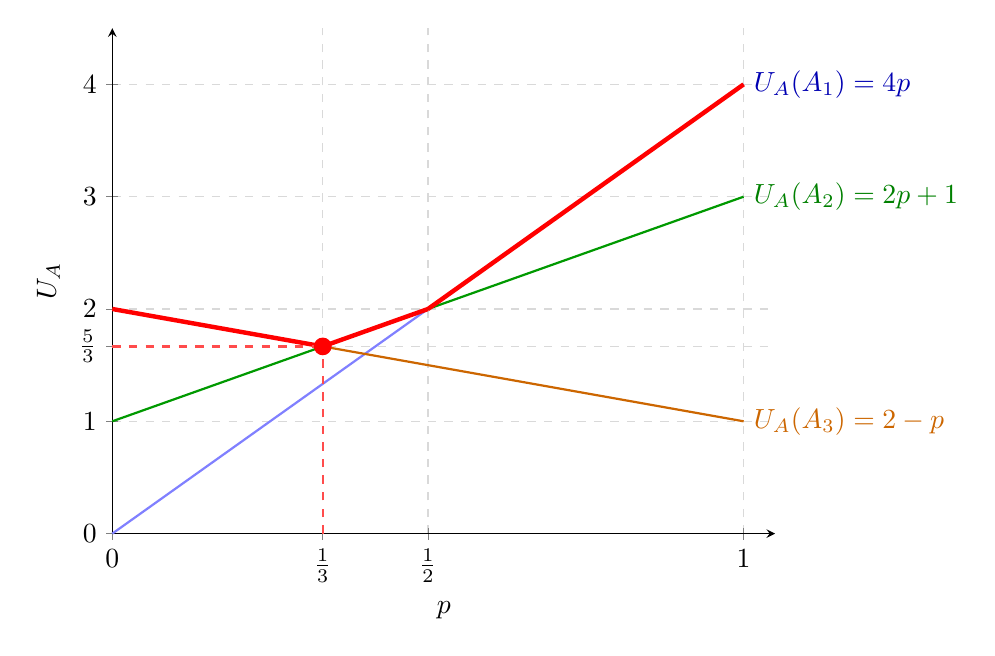
\begin{tikzpicture}
\begin{axis}[
    axis lines = left,
    xlabel = {$p$},
    ylabel = {$U_A$},
    xmin = 0, xmax = 1.05,
    ymin = 0, ymax = 4.5,
    xtick = {0, 0.333, 0.5, 1},
    xticklabels = {$0$, $\frac{1}{3}$, $\frac{1}{2}$, $1$},
    ytick = {0, 1, 1.667, 2, 3, 4},
    yticklabels = {$0$, $1$, $\frac{5}{3}$, $2$, $3$, $4$},
    grid = both,
    grid style = {dashed, gray!30},
    clip = false,
    width = 10cm,
    height = 8cm
]

    % Base lines with labels placed at the right endpoint (p = 1)
    \addplot[domain=0:1, samples=2, blue!50, thick] {4*x}
        node[pos=1, right, blue!70!black] {$U_A(A_1) = 4p$};

    \addplot[domain=0:1, samples=2, green!60!black, thick] {2*x + 1}
        node[pos=1, right, green!50!black] {$U_A(A_2) = 2p + 1$};

    \addplot[domain=0:1, samples=2, orange!80!black, thick] {2 - x}
        node[pos=1, right, orange!80!black] {$U_A(A_3) = 2 - p$};

    % Highlight Upper Envelope (Max for each p) in Red
    \addplot[domain=0:1/3, samples=2, red, ultra thick] {2 - x};
    \addplot[domain=1/3:1/2, samples=2, red, ultra thick] {2*x + 1};
    \addplot[domain=1/2:1, samples=2, red, ultra thick] {4*x};

    % Minimax point only
    \addplot[only marks, mark=*, mark size=3pt, red] coordinates {(1/3, 5/3)};
    \node[above, red, font=\small] at (axis cs:1/3, 1.75) {};

    % Dashed guidelines for minimax point
    \draw[dashed, red!70, thick] (axis cs:1/3, 0) -- (axis cs:1/3, 5/3);
    \draw[dashed, red!70, thick] (axis cs:0, 5/3) -- (axis cs:1/3, 5/3);

\end{axis}
\end{tikzpicture}
\end{document}

        }
        \end{figure}

        \item The bold red line represents the best response for Player A for any mixed strategy \(p\) Player B plays.
        \item Then, for Player B, the best response is at the \textbf{minimax point} \(p^*=\frac{1}{3}\), which minimizes the maximum expected utility for Player A.
        \item From the graph, we know that Player A's best response is a mixed strategy between \(A_2\) and \(A_3\). Let \(q = \sigma_A(A_2)\) and \(1-q = \sigma_A(A_3)\).
        \item In a mixed strategy, Player B must be indifferent between \(B_1\) and \(B_2\). Since \(U_B = -U_A\):
        \[
        U_B(q,B_1) = -3q - 1\cdot(1-q) = q - 2\cdot(1-q) = U_B(q,B_2)
        \]
        Solving, we have \(q^* = \frac{1}{5}\).
    \end{itemize}
\end{itemize}

\end{document}
